%%%%%%%%%%%%%%%%%%%%%%%%%%%%%%%%%%%%%%%%%%%%%%%%
% E.Pinault-Bigeard - s2i@pinault-bigeard.com
% http://s2i.pinault-bigeard.com
% CC BY-NC-SA 2.0 FR - http://creativecommons.org/licenses/by-nc-sa/2.0/fr/
%%%%%%%%%%%%%%%%%%%%%%%%%%%%%%%%%%%%%%%%%%%%%%%%
\documentclass[11pt]{article}

%%%%%%%%%%%%%%%%%%%%%%%%%%%%%%%%%%%%%%%%%%%%%%%%
% Package UPSTI_Document
%%%%%%%%%%%%%%%%%%%%%%%%%%%%%%%%%%%%%%%%%%%%%%%% 
\RequirePackage{UPSTI_Document}

%---------------------------------%
% Paramètres du package
%---------------------------------%

% Version du document (pour la compilation)
% 1: Document prof
% 2: Document élève
% 3: Document à publier
\newcommand{\UPSTIidVersionDocument}{2}

% Choix du type de document
% 2: TD
\newcommand{\UPSTIidTypeDocument}{2}

% Niveau
% 2: PT
\newcommand{\UPSTIidClasse}{2}

% Jean Zay
\newcommand{\UPSTIvariante}{2}

% Titre du document (dans l'en-tête)
\newcommand{\UPSTItitreEnTete}{Résistance des matériaux}      

% Titre
\newcommand{\UPSTItitrePreambule}{TD Transfert}      
\newcommand{\UPSTItitre}{Tracés de diagrammes des efforts intérieurs}      

% Référence au programme
\newcommand{\UPSTIprogramme}{\UPSTIcomp \UPSTIcompP{B1-02}, \UPSTIcompP{B2-49}, \UPSTIcompP{B2-50}, \UPSTIcompP{B2-51}, \UPSTIcompP{C1-07}, \UPSTIcompP{C1-08}}

% Source
%\newcommand{\UPSTIsource}{E.PINAULT-BIGEARD}

% Versioning
\newcommand{\UPSTInumeroVersion}{2.2}
                 
%----------------------------------------------- 
\UPSTIcompileVars		% "Compile" les variables
%%%%%%%%%%%%%%%%%%%%%%%%%%%%%%%%%%%%%%%%%%%%%%%% 


%%%%%%%%%%%%%%%%%%%%%%%%%%%%%%%%%%%%%%%%%%%%%%%% 
% Début du document
%%%%%%%%%%%%%%%%%%%%%%%%%%%%%%%%%%%%%%%%%%%%%%%% 
\begin{document}

% Création de l'en-tête
\UPSTIbuildPage 

\section*{Travail demandé}
\noindent Pour l'ensemble des poutres suivantes:

\UPSTIquestion{Déterminer le torseur de cohésion.}

\UPSTIquestion{Identifier les sollicitations auxquelles est soumise la poutre.}

\UPSTIquestion{Tracer les diagrammes des efforts intérieurs adaptés.}

\UPSTIcorrection{
\UPSTItitreStd{Rappel de la méthode:}
\vspace{-1em}
\begin{enumerate}
\item Identifier les tronçons à étudier
\item Déterminer les actions dans les liaisons (\textbf{si nécessaire}) !
\item Pour chaque tronçon:
\begin{enumerate}
\item Choisir la partie à étudier (gauche/droite)
\item IAME
\item Écrire les éléments de réduction de \tCoh
\end{enumerate}
\item En déduire la ou les sollicitations auxquelles est soumise la poutre.
\end{enumerate}
\vspace{-2em}
}

\section{Exercice 1}
\UPSTIeleveOnly{
\begin{center}
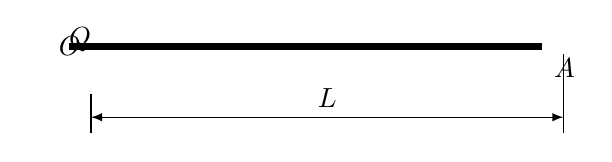
\begin{tikzpicture}
\PoutreEncastrement{0}{0}
\PoutreBaseLocale{6.2}{0.7}
\draw[line width=2.5pt] (0,0) -- (6,0) node[below right] {$A$};
\PoutreCharge{6}{0}{$Q$}
\node at (0,0)[left=0.2] {$O$};
\draw (0,-0.6) -- (0,-1.1);
\draw (6,-0.1) -- (6,-1.1);
\draw[<->,>=latex] (0,-0.9) -- (6,-0.9) node [midway, above] {$L$};
\end{tikzpicture}
\end{center}
}

\UPSTIcorrection{
\vspace{-1em}
\begin{wrapfigure}{r}{9.5cm}
\raggedleft
\vspace{-2em}
\begin{tikzpicture}[black]
% Dessin de la poutre
\PoutreEncastrement{0}{0}
\PoutreBaseLocale{6.2}{0.7}
\draw[line width=2.5pt] (0,0) -- (6,0) node[below right] {$A$};
\PoutreCharge{6}{0}{$Q$}
\node at (0,0)[left=0.2] {$O$};
\draw (0,-0.6) -- (0,-1.1);
\draw (6,-0.1) -- (6,-1.1);
\draw[<->,>=latex] (0,-0.9) -- (6,-0.9) node [midway, above] {$L$};

% Diagrammes des efforts intérieurs
\begin{scope}[yshift=-2cm]
\PoutreDiagCfg[red]

% Diagramme Ty
\begin{scope}
\filldraw[diagCourbe] (0,0) -- (0,-0.5) -- (6,-0.5) -- (6,0) -- cycle ;
\PoutreDiagAxes{$T_y$}{6.2}{-0.8}{0.5}
\draw[diagCourbeAcc] (0,-0.5) -- (6,-0.5);
\draw (-0.1,-0.5) node[left,color=red]{\small{$-Q$}} -- (0.1,-0.5);
\end{scope}

% Diagramme Mfz
\begin{scope}[yshift=-1.7cm]
\filldraw[diagCourbe] (0,0) -- (0,-0.7) -- (6,0) -- cycle ;
\PoutreDiagAxes{\Mfz}{6.2}{-1}{0.5}
\draw[diagCourbeAcc] (0,-0.7) -- (6,0);
\draw (-0.1,-0.7) node[left,color=red]{\small{$-LQ$}} -- (0.1,-0.7);
\end{scope}
\end{scope}
\end{tikzpicture}

\vspace{-16em}
\end{wrapfigure}
\noindent\underline{Tronçon $[OA]$:} $x\in[0,L]$

\noindent $\tCoh=\tAM{\ext}{\text{Droite}}[G]$

\noindent $\UPSTIcadreMathCor{\tCoh=\tColonne{G(x)}{0 \\ -Q \\ 0}{0 \\ 0 \\ -(L-x)Q}{}}$

\vspace{1em}
\noindent La poutre est soumise à de la \UPSTIcadreTextCor{flexion simple}
\vspace{4em}
\pagebreak
}

\section{Exercice 2}
\UPSTIeleveOnly{
\begin{center}
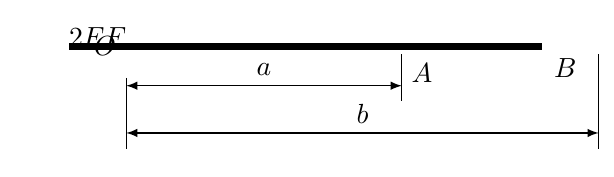
\begin{tikzpicture}
\PoutreEncastrement{0}{0}
\PoutreBaseLocale{6.2}{0.7}
\draw[line width=2.5pt] (0,0) -- (6,0) node[below right] {$B$};
\PoutreCharge{6}{0}{$2F$}
\PoutreCharge{3.5}{0}{$F$}[0][1]
\node at (0,0)[left=0.2] {$O$};
\draw (3.5,-0.1) node[below right] {$A$} -- (3.5,-0.7);
\draw (0,-0.4) -- (0,-1.3);
\draw (6,-0.1) -- (6,-1.3);
\draw[<->,>=latex] (0,-0.5) -- (3.5,-0.5) node [midway, above] {$a$};
\draw[<->,>=latex] (0,-1.1) -- (6,-1.1) node [midway, above] {$b$};
\end{tikzpicture}
\end{center}
}

\UPSTIcorrection{
\vspace{-4em}
\begin{wrapfigure}{r}{9.5cm}
\raggedleft
\begin{tikzpicture}[black]
% Dessin de la poutre
\draw (0,-0.1) -- (0,-1);
\PoutreEncastrement{0}{0}
\PoutreBaseLocale{6.2}{0.7}
\draw[line width=2.5pt] (0,0) -- (6,0) node[below right] {$B$};
\PoutreCharge{6}{0}{$2F$}
\PoutreCharge{3.5}{0}{$F$}[0][1]
\node at (0,0)[left=0.2] {$O$};
\draw (3.5,-0.1) node[below right] {$A$} -- (3.5,-0.7);
\draw (0,-0.4) -- (0,-1.3);
\draw (6,-0.1) -- (6,-1.3);
\draw[<->,>=latex] (0,-0.5) -- (3.5,-0.5) node [midway, above] {$a$};
\draw[<->,>=latex] (0,-1.1) -- (6,-1.1) node [midway, above] {$b$};

% Diagrammes des efforts intérieurs
\begin{scope}[yshift=-2.3cm]
\PoutreDiagCfg[red]

% Diagramme Ty
\begin{scope}
\filldraw[diagCourbe] (0,0) -- (0,-0.5) -- (3.5,-0.5) -- (3.5,-1) -- (6,-1) -- (6,0) -- cycle ;
\PoutreDiagAxes{$T_y$}{6.2}{-1.3}{0.5}
\draw[diagCourbeAcc] (0,-0.5) -- (3.5,-0.5) -- (3.5,-1) -- (6,-1);
\draw (-0.1,-0.5) node[left,color=red]{\small{$-F$}} -- (0.1,-0.5);
\draw (-0.1,-1) node[left,color=red]{\small{$-2F$}} -- (0.1,-1);
\end{scope}

% Diagramme Mfz
\begin{scope}[yshift=-2.3cm]
\filldraw[diagCourbe] (0,0) -- (0,-1) -- (3.5,-0.59) -- (6,0) -- cycle ;
\PoutreDiagAxes{\Mfz}{6.2}{-1.3}{0.5}
\draw[diagCourbeAcc] (0,-1) -- (3.5,-0.59) -- (6,0);
\draw (-0.1,-0.59) node[left,color=red]{\small{$2(a-b)F$}} -- (0.1,-0.59);
\draw (-0.1,-1) node[left,color=red]{\small{$(a-2b)F$}} -- (0.1,-1);
\end{scope}
\end{scope}
\end{tikzpicture}
\vspace{-17em}
\end{wrapfigure}

\noindent\underline{Tronçon $[OA]$:} $x\in[0,a]$

\noindent $\tCoh=\tAM{\ext}{\text{Droite}}[G]$

\noindent $\UPSTIcadreMathCor{\tCoh=\tColonne{G(x)}{0 \\ -F \\ 0}{0 \\ 0 \\ (a-2b+x)F}{}}$

\vspace{1em}
\noindent\underline{Tronçon $[AB]$:} $x\in[a,b]$

\noindent $\tCoh=\tAM{\ext}{\text{Droite}}[G]$

\noindent $\UPSTIcadreMathCor{\tCoh=\tColonne{G(x)}{0 \\ -2F \\ 0}{0 \\ 0 \\ -2(b-x)F}{}}$

\vspace{1em}
\noindent La poutre est soumise à de la \UPSTIcadreTextCor{flexion simple}
}

\section{Exercice 3}
\UPSTIeleveOnly{
\begin{center}
\begin{tikzpicture}[scale=0.9]
\begin{scope}[xshift=8cm]
\setCouleursParametrage{black}{UPSTIcustomColor1}  
\parametrageAngulaireFig{\theta}{\vx{}}{\vy{}}{\vz{}}{\vx{s}}{\vy{s}}[\vz{s}]
\end{scope}
\draw[line width=2.5pt] (3,0) arc (0:90:3);
\PoutreEncastrement{3}{0}[90]
\PoutreCharge{0}{3}{$F$}
\node at (3,0)[above left] {$A$};
\node at (0,3)[left] {$B$};
\node at (0,0)[below right] {$O$};
\draw[->,>=latex] (30:3) --++ (120:1.2) node[right] {\vx{s}};
\draw[->,>=latex] (30:3) -- (30:2) node[above] {\vy{s}};
\draw[->,>=latex] (0,0) -- (60:3) node[midway, left] {$R$};
\node at (28:3)[right] {$G$};
\draw[->,>=latex] (0,0) --++ (-2,0) node[above] {\vy{}};
\draw[->,>=latex] (0,0) --++ (0,2) node[left] {\vx{}};
\draw[dashed] (30:-1.5) -- (30:2);
\draw[->,>=latex] (-1,0) arc (180:210:1) node[midway, left] {$\theta$};
\end{tikzpicture}
\end{center}
}

\UPSTIcorrection{
\vspace{-4em}
\begin{wrapfigure}{r}{6cm}
\raggedleft
\vspace{-2em}
\begin{tikzpicture}[black,scale=0.9]
% Dessin de la poutre
\draw[line width=2.5pt] (3,0) arc (0:90:3);
\PoutreEncastrement{3}{0}[90]
\PoutreCharge{0}{3}{$F$}
\node at (3,0)[above left] {$A$};
\node at (0,3)[left] {$B$};
\node at (0,0)[below right] {$O$};
\draw[->,>=latex] (30:3) --++ (120:1.2) node[right] {\vx{s}};
\draw[->,>=latex] (30:3) -- (30:2) node[above] {\vy{s}};
\draw[->,>=latex] (0,0) -- (60:3) node[midway, left] {$R$};
\node at (28:3)[right] {$G$};
\draw[->,>=latex] (0,0) --++ (-2,0) node[above] {\vy{}};
\draw[->,>=latex] (0,0) --++ (0,2) node[left] {\vx{}};
\draw[dashed] (30:-1.5) -- (30:2);
\draw[->,>=latex] (-1,0) arc (180:210:1) node[midway, left] {$\theta$};

% Diagrammes des efforts intérieurs
\begin{scope}[yshift=-1.3cm]
\PoutreDiagCfg[red]

% Diagramme N
\begin{scope}[xscale=3/90]
\filldraw[diagCourbe] (0,0) -- (0,-1) -- plot [smooth,domain=0:90] (\x,{-cos(\x)}) -- cycle ;
\PoutreDiagAxes{$N$}{96}{-1.3}{0.5}[\theta]
\draw[diagCourbeAcc] plot [smooth,domain=0:90] (\x,{-cos(\x)});
\end{scope}
\draw (-0.1,-1) node[left,color=red]{\small{$-F$}} -- (0.1,-1);

% Diagramme Ty
\begin{scope}[yshift=-3.5cm]
\begin{scope}[xscale=3/90]
\filldraw[diagCourbe] (0,0) -- plot [smooth,domain=0:90] (\x,{sin(\x)}) -- (90,0) -- cycle ;
\PoutreDiagAxes{$T_y$}{96}{-0.2}{1.5}[\theta]
\draw[diagCourbeAcc] plot [smooth,domain=0:90] (\x,{sin(\x)});
\end{scope}
\draw (-0.1,1) node[left,color=red]{\small{$F$}} -- (0.1,1);

% Diagramme Mfz
\begin{scope}[yshift=-2.5cm]
\begin{scope}[xscale=3/90]
\filldraw[diagCourbe] (0,0) -- (0,1.2) -- plot [smooth,domain=0:90] (\x,{1.2*cos(\x)}) -- cycle ;
\PoutreDiagAxes{$\Mfz$}{96}{-0.2}{1.8}[\theta]
\draw[diagCourbeAcc] plot [smooth,domain=0:90] (\x,{1.2*cos(\x)});
\end{scope}
\draw (-0.1,1.2) node[left,color=red]{\small{$FR$}} -- (0.1,1.2);
\end{scope}
\end{scope}
\end{scope}
\end{tikzpicture}
\vspace{-17em}
\end{wrapfigure}

\noindent\underline{Tronçon $AB$:} $\theta\in\left[0,\frac{\pi}{2}\right]$

\noindent $\tCoh=\tAM{\ext}{\text{Droite}}[G]$

\noindent $\Res{\tAM{\ext}{\text{Droite}}}=-F.\vx{}=-F\left(\cos\theta.\vx{s}-\sin\theta.\vy{s}\right)$

\noindent \babarAM{\ext}{\text{Droite}}{G}{B}

\noindent Avec: $\vecteur{GB}=\vecteur{GO}+\vecteur{OB}=R.\vy{s}+R.\vx{}$

\noindent On trouve: $\Mom{G}{\tAM{\ext}{\text{Droite}}}=FR\cos\theta.\vz{}$

\noindent $\UPSTIcadreMathCor{\tCoh=\tColonne{G(\theta)}{-F\cos\theta \\ F\sin\theta \\ 0}{0 \\ 0 \\ FR\cos\theta}{\bB{s}}}$

\vspace{1em}
\noindent La poutre est soumise à de la \UPSTIcadreTextCor{compression} et à de la \UPSTIcadreTextCor{flexion simple}. 

\vspace{5em}
\pagebreak
}

\section{Exercice 4}
\UPSTIeleveOnly{
\begin{center}
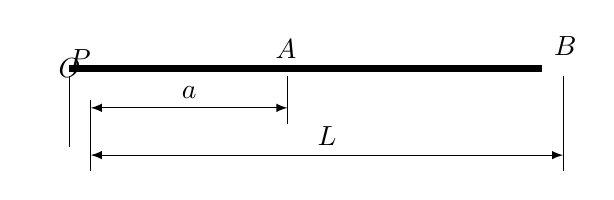
\begin{tikzpicture}
\draw (0,-0.1) -- (0,-1);
\PoutreAppuiSimple{0}{0}
\PoutreAppuiSimple{6}{0}
\PoutreBaseLocale{6.2}{0.2}
\node at (2.5,0)[above right] {$A$};
\draw[line width=2.5pt] (0,0) -- (6,0) node[above right] {$B$};
\PoutreCharge{2.5}{0}{$P$}
\node at (0,0)[above, left=0.2] {$O$};
\draw (2.5,-0.1) -- (2.5,-0.7);
\draw (0,-0.4) -- (0,-1.3);
\draw (6,-0.1) -- (6,-1.3);
\draw[<->,>=latex] (0,-0.5) -- (2.5,-0.5) node [midway, above] {$a$};
\draw[<->,>=latex] (0,-1.1) -- (6,-1.1) node [midway, above] {$L$};
\end{tikzpicture}
\end{center}
}

\UPSTIcorrection{
Il y a 2 tronçons à étudier ($[OA]$ et $[AB]$), mais il est nécessaire au préalable de faire une étude statique pour déterminer les efforts de liaison.

\noindent En utilisant l'équation de moment en \vz{} du PFS appliqué à la poutre, en $O$ puis en $B$, on trouve immédiatement (par la méthode des bras de levier):

\noindent $\UPSTIcadreMathCor{Y_B=\dfrac{a}{L}P}$\quad et \quad $\UPSTIcadreMathCor{Y_O=\left(1-\dfrac{a}{L}\right)P}$

\noindent On peut maintenant passer à l'étude des différents tronçons...

\begin{wrapfigure}{r}{10cm}
\raggedleft
\vspace{-2em}
\begin{tikzpicture}[black]
% Dessin de la poutre
\draw (0,-0.1) -- (0,-1);
\PoutreAppuiSimple{0}{0}
\PoutreAppuiSimple{6}{0}
\PoutreBaseLocale{6.2}{0.2}
\node at (2.5,0)[above right] {$A$};
\draw[line width=2.5pt] (0,0) -- (6,0) node[above right] {$B$};
\PoutreCharge{2.5}{0}{$P$}
\PoutreCharge{0}{0}{$Y_O$}[0][1][red]
\PoutreCharge{6}{0}{$Y_B$}[0][1][red]
\node at (0,0)[above, left=0.2] {$O$};
\draw (2.5,-0.1) -- (2.5,-0.7);
\draw (0,-0.4) -- (0,-1.3);
\draw (6,-0.1) -- (6,-1.3);
\draw[<->,>=latex] (0,-0.5) -- (2.5,-0.5) node [midway, above] {$a$};
\draw[<->,>=latex] (0,-1.1) -- (6,-1.1) node [midway, above] {$L$};

% Diagrammes des efforts intérieurs
\begin{scope}[yshift=-2.9cm]
\PoutreDiagCfg[red]

% Diagramme Ty
\begin{scope}
\filldraw[diagCourbe] (0,0) -- (0,-1+2.5/6) -- (2.5,-1+2.5/6) -- (2.5,2.5/6) -- (6,2.5/6) -- (6,0) -- cycle ;
\PoutreDiagAxes{$T_y$}{6.2}{-0.9}{1}
\draw[diagCourbeAcc] (0,-1+2.5/6) -- (2.5,-1+2.5/6) -- (2.5,2.5/6) -- (6,2.5/6);
\draw (-0.1,2.5/6) node[left,color=red]{\small{$\frac{a}{L}P$}} -- (0.1,2.5/6);
\draw (-0.1,-1+2.5/6) node[left,color=red]{\small{$-\left(1-\frac{a}{L}\right)P$}} -- (0.1,-1+2.5/6);
\end{scope}

% Diagramme Mfz
\begin{scope}[yshift=-3cm]
\filldraw[diagCourbe] plot [smooth,domain=0:2.5] (\x,{0.5*\x*(1-2.5/6)}) -- plot [smooth,domain=2.5:6] (\x,{0.5*(6-\x)*2.5/6}) -- cycle ;
\PoutreDiagAxes{\Mfz}{6.2}{-0.3}{1.3}
\draw[diagCourbeAcc] plot [smooth,domain=0:2.5] (\x,{0.5*\x*(1-2.5/6)}) -- plot [smooth,domain=2.5:6] (\x,{0.5*(6-\x)*2.5/6});
\draw (-0.1,1.25-1.25*2.5/6) node[left,color=red]{\small{$a\left(1-\frac{a}{L}\right)P$}} -- (0.1,1.25-1.25*2.5/6);
\end{scope}
\end{scope}
\end{tikzpicture}
\vspace{-20em}
\end{wrapfigure}

\vspace{2em}
\noindent\underline{Tronçon $[OA]$:} $x\in[0,a]$

\noindent $\tCoh=-\tAM{\ext}{\text{Gauche}}[G]$

\noindent $\UPSTIcadreMathCor{\tCoh=\tColonne{G(x)}{0 \\ -Y_O \\ 0}{0 \\ 0 \\ xY_O}{}}$

\vspace{1em}
\noindent\underline{Tronçon $[AB]$:} $x\in[a,L]$

\noindent $\tCoh=\tAM{\ext}{\text{Droite}}[G]$

\noindent $\UPSTIcadreMathCor{\tCoh=\tColonne{G(x)}{0 \\ Y_B \\ 0}{0 \\ 0 \\ (L-x)Y_B}{}}$

\vspace{1em}
\noindent La poutre est soumise à de la \UPSTIcadreTextCor{flexion simple}
}

\section{Exercice 5}
\UPSTIeleveOnly{
\begin{center}
\begin{tikzpicture}
\draw[line width=2.5pt] (0,0) -- (6,0);
\PoutreRotule{0}{0}
\PoutreAppuiSimple{6}{0}
\PoutreBaseLocale{6.2}{0.2}

\PoutreCharge{2}{0}{$F$}[45][0][UPSTIcustomColor1][1][above]
\draw (1.3,0) arc (180:135:0.7) node[midway, left] {\SI{45}{\degree}};

\PoutreCharge{4}{0}{$F$}

\node at (0,0)[above left] {$A$};
\node at (2,0)[above right] {$B$};
\node at (4.2,0)[above right] {$C$};
\node at (6,0)[above right] {$D$};

\draw (0,-0.9) -- (0,-1.6);
\draw (2,-0.1) -- (2,-1.6);
\draw (4,-0.1) -- (4,-1.6);
\draw (6,-0.9) -- (6,-1.6);
\draw[<->,>=latex] (0,-1.4) --++ (2,0) node [midway, above] {\ofrac{L}{3}};
\draw[<->,>=latex] (2,-1.4) --++ (2,0) node [midway, above] {\ofrac{L}{3}};
\draw[<->,>=latex] (4,-1.4) --++ (2,0) node [midway, above] {\ofrac{L}{3}};
\end{tikzpicture}
\end{center}
}

\UPSTIcorrection{
Il y a 3 tronçons à étudier ($[AB]$, $[BC]$ et $[CD]$), mais il est nécessaire au préalable de faire une étude statique pour déterminer les efforts de liaison.

\noindent En utilisant l'équation de moment en \vz{} du PFS appliqué à la poutre, en $A$ puis en $D$, on trouve immédiatement (par la méthode des bras de levier):

\noindent $\UPSTIcadreMathCor{X_A=-\dfrac{\sqrt{2}}{2}F}$\quad, \quad $\UPSTIcadreMathCor{Y_A=\left(\dfrac{\sqrt{2}}{3}+\dfrac{1}{3}\right)F}$\quad et \quad $\UPSTIcadreMathCor{Y_D=\left(\dfrac{\sqrt{2}}{6}+\dfrac{2}{3}\right)F}$

\pagebreak
\noindent On peut maintenant passer à l'étude des différents tronçons...

\begin{wrapfigure}{r}{10cm}
\raggedleft
\vspace{-2em}
\begin{tikzpicture}[black]
% Dessin de la poutre
\draw[line width=2.5pt] (0,0) -- (6,0);
\PoutreRotule{0}{0}
\PoutreAppuiSimple{6}{0}
\PoutreBaseLocale{6.2}{0.2}

\PoutreCharge{2}{0}{$F$}[45][0][UPSTIcustomColor1][1][above]
\draw (1.3,0) arc (180:135:0.7) node[midway, left] {\SI{45}{\degree}};

\PoutreCharge{4}{0}{$F$}

\node at (0,0)[above left] {$A$};
\node at (2,0)[above right] {$B$};
\node at (4.2,0)[above right] {$C$};
\node at (6,0)[above right] {$D$};

\draw (0,-0.9) -- (0,-1.6);
\draw (2,-0.1) -- (2,-1.6);
\draw (4,-0.1) -- (4,-1.6);
\draw (6,-0.9) -- (6,-1.6);
\draw[<->,>=latex] (0,-1.4) --++ (2,0) node [midway, above] {\ofrac{L}{3}};
\draw[<->,>=latex] (2,-1.4) --++ (2,0) node [midway, above] {\ofrac{L}{3}};
\draw[<->,>=latex] (4,-1.4) --++ (2,0) node [midway, above] {\ofrac{L}{3}};

\PoutreCharge{0}{0}{$Y_A$}[0][1][red]
\PoutreCharge{6}{0}{$Y_D$}[0][1][red]

% Diagrammes des efforts intérieurs
\begin{scope}[yshift=-2.9cm]
\PoutreDiagCfg[red]

% Diagramme N
\begin{scope}
\filldraw[diagCourbe] (0,0) -- (0,0.6) -- (2,0.6) -- (2,0) -- cycle ;
\PoutreDiagAxes{$N$}{6.2}{-0.2}{1}
\draw[diagCourbeAcc] (0,0.6) -- (2,0.6) -- (0,0.6);
\draw (-0.1,0.6) node[left,color=red]{\small{$\frac{\sqrt{2}}{2}F$}} -- (0.1,0.6);
\end{scope}

% Diagramme Ty
\begin{scope}[yshift=-2cm]
\filldraw[diagCourbe] (0,0) -- (0,-0.6) -- (2,-0.6) -- (2,-0.2) -- (4,-0.2) -- (4,0.6) -- (6,0.6) -- (6,0) -- cycle ;
\PoutreDiagAxes{$T_y$}{6.2}{-0.9}{1}
\draw[diagCourbeAcc] (0,-0.6) -- (2,-0.6) -- (2,-0.2) -- (4,-0.2) -- (4,0.6) -- (6,0.6);

\draw (-0.1,-0.6)  -- (0.1,-0.6);
\draw (-0.1,-0.9) node[left,color=red]{\small{$-\left(\frac{\sqrt{2}}{3}+\frac{1}{3}\right)F$}};
\draw (-0.1,0.6) node[left,color=red]{\small{$\left(\frac{\sqrt{2}}{6}+\frac{2}{3}\right)F$}} -- (0.1,0.6);
\draw (-0.1,-0.2) node[left,color=red]{\small{$\left(\frac{\sqrt{2}}{6}-\frac{1}{3}\right)F$}} -- (0.1,-0.2);


% Diagramme Mfz
\begin{scope}[yshift=-3.2cm]
\filldraw[diagCourbe] plot [smooth,domain=0:2] (\x,{(sqrt(2)/3+1/3)*\x*(0.5}) -- plot [smooth,domain=2:4] (\x,{1/3*(\x+sqrt(2)/2*(6-\x))*(0.5)}) -- plot [smooth,domain=4:6] (\x,{(sqrt(2)/6+2/3)*(6-\x)*(0.5}) -- cycle ;
\PoutreDiagAxes{\Mfz}{6.2}{-0.2}{1.5}
\draw[diagCourbeAcc] plot [smooth,domain=0:2] (\x,{(sqrt(2)/3+1/3)*\x*(0.5}) -- plot [smooth,domain=2:4] (\x,{1/3*(\x+sqrt(2)/2*(6-\x))*(0.5)}) -- plot [smooth,domain=4:6] (\x,{(sqrt(2)/6+2/3)*(6-\x)*(0.5});
\draw (-0.1,0.9) -- (0.1,0.9);
\draw (-0.1,1.1) node[left,color=red]{\small{$\left(\frac{\sqrt{2}}{6}+\frac{2}{3}\right)F\frac{L}{3}$}};
\draw (-0.1,0.8) -- (0.1,0.8);
\draw (-0.1,0.4) node[left,color=red]{\small{$\left(\frac{\sqrt{2}}{3}+\frac{1}{3}\right)F\frac{L}{3}$}};
\end{scope}
\end{scope}
\end{scope}
\end{tikzpicture}
\vspace{-20em}
\end{wrapfigure}

\vspace{2em}
\noindent\underline{Tronçon $[AB]$:} $x\in[0,L/3]$

\noindent $\tCoh=-\tAM{\ext}{\text{Gauche}}[G]$

\noindent $\tCoh=\tCohesionCan{1}{1}{0}{0}{0}{1}$ \quad avec:

\noindent $\UPSTIcadreMathCor{N=\frac{\sqrt{2}}{2}F}$ \quad $\UPSTIcadreMathCor{T_y=-\left(\frac{\sqrt{2}}{3}+\frac{1}{3}\right)F}$

\noindent $\UPSTIcadreMathCor{\Mfz=\left(\frac{\sqrt{2}}{3}+\frac{1}{3}\right)Fx}$


\vspace{1em}
\noindent\underline{Tronçon $[BC]$:} $x\in[L/3,2L/3]$

\noindent $\tCoh=\tAM{\ext}{\text{Droite}}[G]$

\noindent $\UPSTIcadreMathCor{N=0}$ \quad $\UPSTIcadreMathCor{T_y=\left(\frac{\sqrt{2}}{6}-\frac{1}{3}\right)F}$ 

\noindent $\UPSTIcadreMathCor{\Mfz=\frac{1}{3}F\left(x+\frac{\sqrt{2}}{2}(L-x)\right)}$

\vspace{1em}
\noindent\underline{Tronçon $[CD]$:} $x\in[2L/3,L]$

\noindent $\tCoh=\tAM{\ext}{\text{Droite}}[G]$

\noindent $\UPSTIcadreMathCor{N=0}$ \quad $\UPSTIcadreMathCor{T_y=\left(\frac{\sqrt{2}}{6}+\frac{2}{3}\right)F}$ \quad $\UPSTIcadreMathCor{\Mfz=\left(\frac{\sqrt{2}}{6}+\frac{2}{3}\right)F(L-x)}$

\vspace{1em}
\noindent La poutre est soumise à de la \UPSTIcadreTextCor{traction} et de la \UPSTIcadreTextCor{flexion simple}.
\vspace{-1em}
}

\section{Exercice 6}
\UPSTIeleveOnly{
\vspace{-1em}
\begin{center}
\begin{tikzpicture}
\begin{scope}[xshift=4.5cm,yshift=0.3cm,scale=0.8]
\setCouleursParametrage{black}{UPSTIcustomColor1}  
\parametrageAngulaireFig{\theta}{\vx{}}{\vy{}}{\vz{}}{\vx{s}}{\vy{s}}[\vz{s}]
\end{scope}

\draw[line width=2.5pt] (0,0) arc (-70:250:2);
\PoutreCharge{0}{0}{$P$}[-90][1][UPSTIcustomColor1][1][above]
\PoutreCharge{-1.38608}{0}{$P$}[90][1][UPSTIcustomColor1][1][above]
\draw[dashed] (0,0) --++ (2,0) node[name=fl] {};
\begin{scope}[shift={(110:2)}]
\node at (-70:2)[left] {$A$};
\node at (-110:2)[right] {$B$};
\draw[->,>=latex] (0,0) --++ (150:2) node[midway, above right] {$R$};
\draw (0,0) node[above right] {$C$};
\draw[->,>=latex] (0,0) --++ (-2.5,0) node[above] {\vy{}};
\draw[->,>=latex] (0,0) --++ (0,2.5) node[right] {\vx{}};
\fill[white] (0,0) circle (0.13);
\draw [very thick] (0,0) circle (0.13);
\fill[black] (0,0) circle (0.03);
\draw [->,thick] (0,0) circle (0.04);
\node[below=0.5em] at (0,0) {$\vz{}=\vz{s}$};
\draw[dashed] (0,0) -- (2.7,0);
\draw[<->,>=latex] (2.6,0) -- ($(fl.center)+(-0.08,0)$) node[midway, right] {$a$};
\begin{scope}[shift={(30:2)},rotate=30]
\draw[->,>=latex] (0,0) --++ (-1,0) node[above] {\vy{s}};
\draw[->,>=latex] (0,0) --++ (0,1.2) node[right] {\vx{s}};
\node at (0,0)[right] {$G$};
\end{scope}
\end{scope}
\end{tikzpicture}
\end{center}
}

\UPSTIcorrection{
\vspace{-5em}
\begin{center}
\begin{tikzpicture}[black,scale=0.9]
% Dessin de la poutre
\begin{scope}[xshift=4.5cm,yshift=0.3cm,scale=0.9]
\setCouleursParametrage{black}{UPSTIcustomColor1}  
\parametrageAngulaireFig{\theta}{\vx{}}{\vy{}}{\vz{}}{\vx{s}}{\vy{s}}[\vz{s}]
\end{scope}

\draw[line width=2.5pt] (0,0) arc (-70:250:2);
\PoutreCharge{0}{0}{$P$}[-90][1][UPSTIcustomColor1][1][above]
\PoutreCharge{-1.38608}{0}{$P$}[90][1][UPSTIcustomColor1][1][above]
\draw[dashed] (0,0) --++ (2,0) node[name=fl] {};
\begin{scope}[shift={(110:2)}]
\node at (-70:2)[left] {$A$};
\node at (-110:2)[right] {$B$};
\draw[->,>=latex] (0,0) --++ (150:2) node[midway, above right] {$R$};
\draw (0,0) node[above right] {$C$};
\draw[->,>=latex] (0,0) --++ (-2.5,0) node[above] {\vy{}};
\draw[->,>=latex] (0,0) --++ (0,2.5) node[right] {\vx{}};
\fill[white] (0,0) circle (0.13);
\draw [very thick] (0,0) circle (0.13);
\fill[black] (0,0) circle (0.03);
\draw [->,thick] (0,0) circle (0.04);
\node[below=0.5em] at (0,0) {$\vz{}=\vz{s}$};
\draw[dashed] (0,0) -- (2.7,0);
\draw[<->,>=latex] (2.6,0) -- ($(fl.center)+(-0.08,0)$) node[midway, right] {$a$};
\begin{scope}[shift={(30:2)},rotate=30]
\draw[->,>=latex] (0,0) --++ (-1,0) node[above] {\vy{s}};
\draw[->,>=latex] (0,0) --++ (0,1.2) node[right] {\vx{s}};
\node at (0,0)[right] {$G$};
\end{scope}
\end{scope}
\end{tikzpicture}
\end{center}

\pagebreak
\begin{wrapfigure}{r}{8.5cm}
\centering
\vspace{-2em}
\begin{tikzpicture}[black,scale=0.9]
% Diagrammes des efforts intérieurs
\begin{scope}
\PoutreDiagCfg[red]

% Diagramme N
\begin{scope}[xscale=6/320]
\filldraw[diagCourbe] (-70,0) -- (-70,{sin(-70)}) -- plot [smooth,domain=-70:250] (\x,{sin(\x)}) -- (250,{sin(250)}) -- (250,0) -- cycle ;
\draw[->,>=latex] (0,-1.2) -- (0,1.5) node[left] {$N$};
\draw[->,>=latex] (-86,0) -- (314,0) node[right] {$\theta$};

\draw[diagCourbeAcc] (-70,0) -- plot [smooth,domain=-70:250] (\x,{sin(\x)}) -- (250,0);
\draw (90,-0.1) node[below,color=red]{\small{$\frac{\pi}{2}$}} -- (90,0.1);
\end{scope}
\draw (-0.1,-1) node[left,color=red]{\small{$-F$}} -- (0.1,-1);
\draw (-0.1,1) node[left,color=red]{\small{$F$}} -- (0.1,1);

% Diagramme Ty
\begin{scope}[yshift=-3.5cm]
\begin{scope}[xscale=6/320]
\filldraw[diagCourbe] (-70,0) -- (-70,{cos(-70)}) -- plot [smooth,domain=-70:250] (\x,{cos(\x)}) -- (250,{cos(250)}) -- (250,0) -- cycle ;
\draw[->,>=latex] (0,-1.2) -- (0,1.5) node[left] {$T_y$};
\draw[->,>=latex] (-86,0) -- (314,0) node[right] {$\theta$};

\draw[diagCourbeAcc] (-70,0) -- plot [smooth,domain=-70:250] (\x,{cos(\x)}) -- (250,0);
\draw (90,-0.1) node[above right,color=red]{\small{$\frac{\pi}{2}$}} -- (90,0.1);
\end{scope}
\draw (-0.1,-1) node[below left,color=red]{\small{$-F$}} -- (0.1,-1);
\draw (-0.1,1) node[left=1em,color=red]{\small{$F$}} -- (0.1,1);

% Diagramme Mfz
\begin{scope}[yshift=-3.1cm]
\begin{scope}[xscale=6/320]
\filldraw[diagCourbe] (-70,0) -- (-70,{-0.6-sin(-70)}) -- plot [smooth,domain=-70:250] (\x,{-0.6-sin(\x)}) -- (250,{-0.6-sin(250)}) -- (250,0) -- cycle ;
\draw[->,>=latex] (0,-1.8) -- (0,1.1) node[left] {$\Mfz$};
\draw[->,>=latex] (-86,0) -- (314,0) node[right] {$\theta$};

\draw[diagCourbeAcc]  (-70,0) -- plot [smooth,domain=-70:250] (\x,{-0.6-sin(\x)}) -- (250,0);

\draw (90,-0.1) -- (90,0.1);
\end{scope}
\draw (-0.1,-1.6) node[left,color=red]{\small{$-P(a+R)$}} -- (0.1,-1.6);
\draw (-0.1,0.4) -- (0.1,0.4) node[right,color=red]{\small{$-P(a-R)\quad (a<R)$}};


\end{scope}
\end{scope}
\end{scope}
\end{tikzpicture}
\vspace{-8em}
\end{wrapfigure}
\noindent\underline{Tronçon $AB$:}

\noindent $\tCoh=\tAM{\ext}{\text{Droite}}[G]$

\noindent $\Res{\tAM{\ext}{\text{Droite}}}=P\vy{}=P(\sin\theta.\vx{s}+\cos\theta.\vy{s})$

\noindent \babarAM{\ext}{\text{Droite}}{G}{B}

\noindent Avec: $\vecteur{GB}=\vecteur{GC}+\vecteur{CB}=R.\vy{s}-a.\vx{}+k.\vy{}$

\noindent On trouve: $\Mom{G}{\tAM{\ext}{\text{Droite}}}=-P(a+R\sin\theta).\vz{}$

\noindent $\UPSTIcadreMathCor{\tCoh=\tColonne{G(\theta)}{P\sin\theta \\ P\cos\theta \\ 0}{0 \\ 0 \\ -P(a+R\sin\theta)}{\bB{s}}}$

\vspace{1em}
\noindent La poutre est soumise à de la \UPSTIcadreTextCor{compression} et à de la \UPSTIcadreTextCor{flexion simple} (c'est l'étude d'un circlips !). 
\vspace{-1em}
}

\section{Exercice 7}
\UPSTIeleveOnly{
\begin{center}
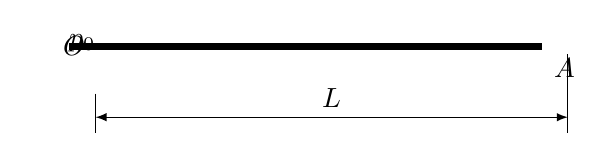
\begin{tikzpicture}
\PoutreEncastrement{0}{0}
\PoutreBaseLocale{6.2}{0.7}
\draw[line width=2.5pt] (0,0) -- (6,0) node[below right] {$A$};
\PoutreChargeRepartie{0}{0}{6}{$p_0$}
\node at (0,0)[left=0.2] {$O$};
\draw (0,-0.6) -- (0,-1.1);
\draw (6,-0.1) -- (6,-1.1);
\draw[<->,>=latex] (0,-0.9) -- (6,-0.9) node [midway, above] {$L$};
\end{tikzpicture}
\end{center}
}

\UPSTIcorrection{
\noindent On doit tout d'abord trouver le modèle global de la charge répartie:
\vspace{-1em}
\begin{center}
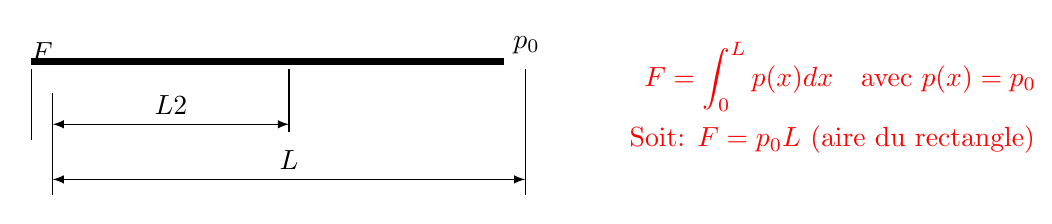
\begin{tikzpicture}[black]
\draw (0,-0.1) -- (0,-1);
\PoutreChargeRepartie{0}{0}{6}{}
\draw[line width=2.5pt] (0,0) -- (6,0);
\node at (6,0.2)[right] {$p_0$};
\PoutreCharge{3}{0}{$F$}[0][0][red]
\draw (3,-0.1) -- (3,-0.9);
\draw (0,-0.4) -- (0,-1.7);
\draw (6,-0.1) -- (6,-1.7);
\draw[<->,>=latex] (0,-0.8) -- (3,-0.8) node [midway, above] {$\ofrac{L}{2}$};
\draw[<->,>=latex] (0,-1.5) -- (6,-1.5) node [midway, above] {$L$};

\node at (10,-0.2)[red] {$\displaystyle F=\int_0^L p(x)dx$\quad avec $p(x)=p_0$};
\node at (9.9,-1)[red] {Soit: $F=p_0L$ (aire du rectangle)};

\end{tikzpicture}
\end{center}

\noindent On peut ensuite déterminer le torseur de cohésion:

\begin{wrapfigure}{r}{9.5cm}
\raggedleft
\vspace{-4em}
\begin{tikzpicture}[black]
% Dessin de la poutre
\PoutreEncastrement{0}{0}
\PoutreBaseLocale{6.2}{0.7}
\draw[line width=2.5pt] (0,0) -- (6,0) node[below right] {$A$};
\PoutreChargeRepartie{0}{0}{6}{$p_0$}
\node at (0,0)[left=0.2] {$O$};
\draw (0,-0.6) -- (0,-1.1);
\draw (6,-0.1) -- (6,-1.1);
\draw[<->,>=latex] (0,-0.9) -- (6,-0.9) node [midway, above] {$L$};

% Diagrammes des efforts intérieurs
\begin{scope}[yshift=-2cm]
\PoutreDiagCfg[red]

% Diagramme Ty
\begin{scope}
\filldraw[diagCourbe] (0,0) -- (0,-0.7) -- (6,0) -- cycle ;
\PoutreDiagAxes{$T_y$}{6.2}{-1}{0.5}
\draw[diagCourbeAcc] (0,-0.7) -- (6,0);
\draw (-0.1,-0.7) node[left,color=red]{\small{$-p_0L$}} -- (0.1,-0.7);
\end{scope}

% Diagramme Mfz
\begin{scope}[yshift=-2cm]
\filldraw[diagCourbe] (0,0) -- (0,-1.5) -- plot [smooth,domain=0:6] (\x,{-1.5/36*(6-\x)^2}) -- (6,0) -- cycle ;
\PoutreDiagAxes{\Mfz}{6.2}{-1.8}{0.5}
\draw[diagCourbeAcc] (0,-1.5) -- plot [smooth,domain=0:6] (\x,{-1.5/36*(6-\x)^2}) -- (6,0);
\draw (-0.1,-1.5) node[left,color=red]{\small{$-\dfrac{p_0L^2}{2}$}} -- (0.1,-1.5);
\end{scope}
\end{scope}
\end{tikzpicture}
\vspace{-17em}
\end{wrapfigure}

\noindent\underline{Tronçon $[OA]$:} $x\in[0,L]$

\noindent $\tCoh=\tAM{\ext}{\text{Droite}}[G]$

\noindent $\UPSTIcadreMathCor{\tCoh=\tColonne{G(x)}{0 \\ -p_0(L-x) \\ 0}{0 \\ 0 \\ -\dfrac{p_0}{2}(L-x)^2}{}}$

\vspace{1em}
\noindent La poutre est soumise à de la \UPSTIcadreTextCor{flexion simple}

\vspace{5em}
\pagebreak
}

\UPSTIeleveOnly{\vspace{0.5em}}
\section{Exercice 8}
\UPSTIeleveOnly{
\begin{center}
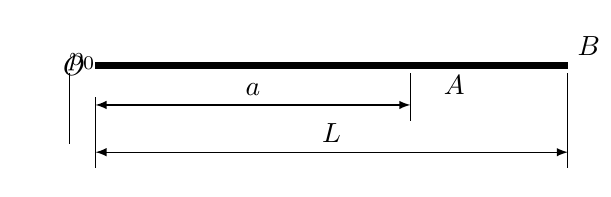
\begin{tikzpicture}
\draw (0,-0.1) -- (0,-1);
\PoutreAppuiSimple{0}{0}
\PoutreAppuiSimple{4}{0}
\PoutreBaseLocale{6.2}{0.6}
\PoutreChargeRepartie{0}{0}{6}{$p_0$}
\node at (4.3,0)[below right] {$A$};
\node at (6,0)[above right] {$B$};
\draw[line width=2.5pt] (0,0) -- (6,0);
\node at (0,0)[above, left=0.2] {$O$};
\draw (4,-0.1) -- (4,-0.7);
\draw (0,-0.4) -- (0,-1.3);
\draw (6,-0.1) -- (6,-1.3);
\draw[<->,>=latex] (0,-0.5) -- (4,-0.5) node [midway, above] {$a$};
\draw[<->,>=latex] (0,-1.1) -- (6,-1.1) node [midway, above] {$L$};
\end{tikzpicture}
\end{center}
}

\UPSTIcorrection{
Il y a 2 tronçons à étudier ($[OA]$ et $[AB]$), mais il est nécessaire au préalable de faire une étude statique pour déterminer les efforts de liaison.

\noindent En utilisant l'équation de moment en \vz{} du PFS appliqué à la poutre, en $O$ puis en $A$, on trouve immédiatement (par la méthode des bras de levier):

\noindent $\UPSTIcadreMathCor{Y_A=p_0\dfrac{L^2}{2a}}$\quad et \quad $\UPSTIcadreMathCor{Y_O=p_0L\left(1-\dfrac{L}{2a}\right)}$

\noindent On peut maintenant passer à l'étude des différents tronçons...

\begin{wrapfigure}{r}{10.5cm}
\raggedleft
\vspace{0em}
\begin{tikzpicture}[black]
% Dessin de la poutre
\draw (0,-0.1) -- (0,-1);
\PoutreAppuiSimple{0}{0}
\PoutreAppuiSimple{4}{0}
\PoutreBaseLocale{5.5}{0.6}
\PoutreChargeRepartie{0}{0}{6}{$p_0$}
\node at (4.3,0)[below right] {$A$};
\node at (6,0)[above right] {$B$};
\draw[line width=2.5pt] (0,0) -- (6,0);
\node at (0,0)[above, left=0.2] {$O$};
\PoutreCharge{0}{0}{$Y_O$}[0][1][red]
\PoutreCharge{4}{0}{$Y_A$}[0][1][red]
\draw (4,-0.1) -- (4,-0.7);
\draw (0,-0.4) -- (0,-1.3);
\draw (6,-0.1) -- (6,-1.3);
\draw[<->,>=latex] (0,-0.5) -- (4,-0.5) node [midway, above] {$a$};
\draw[<->,>=latex] (0,-1.1) -- (6,-1.1) node [midway, above] {$L$};

% Diagrammes des efforts intérieurs
\begin{scope}[yshift=-3.1cm]
\PoutreDiagCfg[red]

% Diagramme Ty
\begin{scope}
\filldraw[diagCourbe] (0,0) -- (0,-0.3*1.5) -- plot [smooth,domain=0:4] (\x,{-0.3*(1.5-\x)}) -- plot [smooth,domain=4:6] (\x,{-0.3*(6-\x)}) -- cycle ;
\PoutreDiagAxes{$T_y$}{5.5}{-0.9}{1.2}
\draw[diagCourbeAcc] plot [smooth,domain=0:4] (\x,{-0.3*(1.5-\x)}) -- plot [smooth,domain=4:6] (\x,{-0.3*(6-\x)});
\draw (-0.1,-0.3*2) node[left,color=red]{\small{$p_0(L-a)$}} -- (0.1,-0.3*2);
\draw (-0.1,-0.3*1.5) node[above left,color=red]{\small{$p_0L\left(1-\frac{L}{2a}\right)$}} -- (0.1,-0.3*1.5);
\draw (-0.1,0.3*2.5) node[left,color=red]{\small{$p_0\left[a-L\left(1-\frac{L}{2a}\right)\right]$}} -- (0.1,0.3*2.5);
\end{scope}

% Diagramme Mfz
\begin{scope}[yshift=-3.2cm]
\filldraw[diagCourbe] plot [smooth,domain=0:4] (\x,{0.4*(-1/2*\x^2+3/2*\x)}) -- plot [smooth,domain=4:6] (\x,{-0.4*1/2*(6-\x)^2}) -- cycle ;
\PoutreDiagAxes{\Mfz}{5.5}{-1}{0.8}
\draw[diagCourbeAcc] plot [smooth,domain=0:4] (\x,{0.4*(-1/2*\x^2+3/2*\x)}) -- plot [smooth,domain=4:6] (\x,{-0.4*1/2*(6-\x)^2});
\draw[<->,>=latex,red] (0.8,0.47) --++ (1.4,0);
\draw (-0.1,-0.8) node[left,color=red]{\small{$-\frac{p_0}{2}(L-a)^2$}} -- (0.1,-0.8);
\end{scope}
\end{scope}
\end{tikzpicture}
\vspace{-20em}
\end{wrapfigure}

\vspace{2em}
\noindent\underline{Tronçon $[OA]$:} $x\in[0,a]$

\noindent $\tCoh=-\tAM{\ext}{\text{Gauche}}[G]$

\noindent $\tCoh=\tCohesionCan{0}{1}{0}{0}{0}{1}$ \quad avec:

\noindent $\UPSTIcadreMathCor{T_y=p_0x-Y_O}$

\noindent $\UPSTIcadreMathCor{\Mfz=-\dfrac{x^2}{2}p_0+xY_O}$

\vspace{1em}
\noindent\underline{Tronçon $[AB]$:} $x\in[a,L]$

\noindent $\tCoh=\tAM{\ext}{\text{Droite}}[G]$

\noindent $\UPSTIcadreMathCor{T_y=p_0(L-x)}$

\noindent $\UPSTIcadreMathCor{\Mfz=\dfrac{p_0}{2}(L-x)^2}$

\vspace{1em}
\noindent La poutre est soumise à de la \UPSTIcadreTextCor{flexion simple}
}


\UPSTIeleveOnly{\vspace{0.5em}}
\section{Exercice 9}
\UPSTIeleveOnly{
\vspace{-1.1em}
\begin{center}
\begin{tikzpicture}
\PoutreAppuiSimple{4}{0}
\PoutreBaseLocale{6.2}{0.2}
\PoutreChargeRepartie{2}{0}{4}{}[0][UPSTIcustomColor1][0.8]
\fill[white] (2,0) -- (6,0.8) -- (6,1) -- (1.5,1)  -- (1.5,0) -- cycle ;
\draw[UPSTIcustomColor1] (2,0)--(6,0.8) node[below right] {\small $p_0$};
\draw[line width=2.5pt] (0,0) -- (6,0);
\PoutreRotule{0}{0}
\node at (2,0)[above] {$A$};
\node at (4.2,0)[below right] {$B$};
\node at (6,0)[below right] {$C$};
\node at (0,0)[above, left=0.2] {$O$};
\draw (0,-0.9) -- (0,-1.6);
\draw (2,-0.1) -- (2,-1.6);
\draw (4,-0.9) -- (4,-1.6);
\draw (6,-0.1) -- (6,-1.6);
\draw[<->,>=latex] (0,-1.4) -- (2,-1.4) node [midway, above] {\ofrac{a}{2}};
\draw[<->,>=latex] (2,-1.4) -- (4,-1.4) node [midway, above] {\ofrac{a}{2}};
\draw[<->,>=latex] (4,-1.4) -- (6,-1.4) node [midway, above] {\ofrac{a}{2}};
\end{tikzpicture}
\end{center}
}

\UPSTIcorrection{
Il y a 3 tronçons à étudier ($[OA]$, $[AB]$ et $[BC]$), mais il est nécessaire au préalable de faire une étude statique pour déterminer les efforts de liaison.

\noindent On peut trouver le modèle global d'une charge répartie:
\vspace{-1em}
\begin{center}
\begin{tikzpicture}[black]
\begin{scope}[xshift=-2cm]
\PoutreChargeRepartie{2}{0}{4}{}[0][UPSTIcustomColor1][0.8]
\fill[white] (2,0) -- (6,0.8) -- (6,1) -- (1.5,1)  -- (1.5,0) -- cycle ;
\draw[UPSTIcustomColor1] (2,0)--(6,0.8) node[below right] {\small $p_0$};
\draw[line width=2.5pt] (2,0) -- (6,0);
\draw (2,-0.1) -- (2,-1.4);
\draw (4.66,-0.1) -- (4.66,-0.9);
\draw (6,-0.1) -- (6,-1.4);
\PoutreCharge{4.66}{0}{$F_1$}[0][0][red]
\draw[<->,>=latex] (2,-0.7) -- (4.66,-0.7) node [midway, above] {\ofrac{2a}{3}};
\draw[<->,>=latex] (2,-1.2) -- (6,-1.2) node [midway, above] {$a$};
\end{scope}

\begin{scope}[xshift=6cm]
\PoutreChargeRepartie{2}{0}{2.6}{}[0][UPSTIcustomColor1][0.52]
\fill[white] (2,0) -- (6,0.8) -- (6,1) -- (1.5,1)  -- (1.5,0) -- cycle ;
\draw[UPSTIcustomColor1,dashed] (4.6,0.52) --(6,0.8) node[below right] {\small $p_0$} -- (6,0);
\draw[UPSTIcustomColor1] (2,0) -- (4.6,0.52) node[below right] {\small $h$} -- (4.6,0);
\draw[line width=2.5pt] (2,0) -- (6,0);
\draw (2,-0.1) -- (2,-1.9);
\draw (3.73,-0.1) -- (3.73,-0.9);
\draw (4.6,-0.1) -- (4.6,-1.4);
\draw (6,-0.1) -- (6,-1.9);
\PoutreCharge{3.73}{0}{$F_2$}[0][0][red]
\draw[<->,>=latex] (2,-0.7) -- (3.73,-0.7) node [midway, above] {\ofrac{2x}{3}};
\draw[<->,>=latex] (2,-1.2) -- (4.6,-1.2) node [midway, above] {$x$};
\draw[<->,>=latex] (2,-1.7) -- (6,-1.7) node [midway, above] {$a$};
\end{scope}
\end{tikzpicture}
\end{center}

\noindent Dans le premier cas, l'intensité de la résultante est égale à l'aire du triangle, à savoir $F_1=\dfrac{p_0}{2}a$.

\noindent Pour le deuxième cas, utile lors de la recherche de l'expression du torseur de cohésion, il faut dans un premier temps utiliser Thalès pour déterminer $h=\dfrac{p_0}{a}x$. Dès lors, on calcule l'aire du triangle en conséquence: \linebreak $F_2=\dfrac{p_0}{2a}x^2$.

\noindent En utilisant l'équation de moment en \vz{} du PFS appliqué à la poutre, en $O$ puis en $A$, on trouve alors (par la méthode des bras de levier):

\noindent $\UPSTIcadreMathCor{Y_B=\dfrac{7a}{12}p_0}$ \qquad $\UPSTIcadreMathCor{Y_O=-\dfrac{a}{12}p_0}$ \quad et \quad $\UPSTIcadreMathCor{X_O=0}$

\noindent On peut maintenant passer à l'étude des différents tronçons...

\begin{wrapfigure}{r}{10.5cm}
\raggedleft
\vspace{0em}
\begin{tikzpicture}[black]
% Dessin de la poutre
\PoutreAppuiSimple{4}{0}
\PoutreBaseLocale{6.2}{0.2}
\PoutreChargeRepartie{2}{0}{4}{}[0][UPSTIcustomColor1][0.8]
\fill[white] (2,0) -- (6,0.8) -- (6,1) -- (1.5,1)  -- (1.5,0) -- cycle ;
\draw[UPSTIcustomColor1] (2,0)--(6,0.8) node[below right] {\small $p_0$};
\draw[line width=2.5pt] (0,0) -- (6,0);
\PoutreRotule{0}{0}
\node at (2,0)[above] {$A$};
\node at (4.2,0)[below right] {$B$};
\node at (6,0)[below right] {$C$};
\node at (0,0)[above, left=0.2] {$O$};
\draw (0,-0.9) -- (0,-1.6);
\draw (2,-0.1) -- (2,-1.6);
\draw (4,-0.9) -- (4,-1.6);
\draw (6,-0.1) -- (6,-1.6);
\draw[<->,>=latex] (0,-1.4) -- (2,-1.4) node [midway, above] {\ofrac{a}{2}};
\draw[<->,>=latex] (2,-1.4) -- (4,-1.4) node [midway, above] {\ofrac{a}{2}};
\draw[<->,>=latex] (4,-1.4) -- (6,-1.4) node [midway, above] {\ofrac{a}{2}};
\PoutreCharge{0}{0}{$Y_O$}[0][1][red]
\PoutreCharge{4}{0}{$Y_A$}[0][1][red]

% Diagrammes des efforts intérieurs
\begin{scope}[yshift=-3.4cm]
\PoutreDiagCfg[red]

% Diagramme Ty
\begin{scope}
\filldraw[diagCourbe] (0,0) -- (0,1/3) -- (2,1/3) -- plot [smooth,domain=2:4] (\x,{1/8*\x^2-1/2*\x+5/6}) -- plot [smooth,domain=4:6] (\x,{1/8*\x^2-1/2*\x-3/2}) -- cycle ;
\PoutreDiagAxes{$T_y$}{6.2}{-1.8}{1.2}
\draw[diagCourbeAcc] (0,1/3) -- (2,1/3) -- plot [smooth,domain=2:4] (\x,{1/8*\x^2-1/2*\x+5/6}) -- plot [smooth,domain=4:6] (\x,{1/8*\x^2-1/2*\x-3/2});
\draw (-0.1,5/6) node[left,color=red]{\small{$\frac{5a}{24}p_0$}} -- (0.1,5/6);
\draw (-0.1,1/3) node[left,color=red]{\small{$\frac{a}{12}p_0$}} -- (0.1,1/3);
\draw (-0.1,-1.5) node[left,color=red]{\small{$-\frac{3a}{8}p_0$}} -- (0.1,-1.5);
\end{scope}

% Diagramme Mfz
\begin{scope}[yshift=-2.8cm]
\filldraw[diagCourbe] plot [smooth,domain=0:2] (\x,{-1/3*\x}) -- plot [smooth,domain=2:4] (\x,{-1/24*\x^3+1/4*\x^2-5/6*\x+1/3}) -- plot [smooth,domain=4:6] (\x,{-1/24*\x^3+1/4*\x^2+3/2*\x-9}) -- cycle ;
\PoutreDiagAxes{\Mfz}{6.2}{-2}{0.5}
\draw[diagCourbeAcc] plot [smooth,domain=0:2] (\x,{-1/3*\x}) -- plot [smooth,domain=2:4] (\x,{-1/24*\x^3+1/4*\x^2-5/6*\x+1/3}) -- plot [smooth,domain=4:6] (\x,{-1/24*\x^3+1/4*\x^2+3/2*\x-9});
\draw (-0.1,-5/3) node[left,color=red]{\small{$-\frac{5a^2}{48}p_0$}} -- (0.1,-5/3);
\end{scope}
\end{scope}
\end{tikzpicture}
\vspace{-20em}
\end{wrapfigure}

\vspace{2em}
\noindent\underline{Tronçon $[OA]$:} $x\in\left[0,\frac{a}{2}\right]$

\noindent $\tCoh=-\tAM{\ext}{\text{Gauche}}[G]$

\noindent $\UPSTIcadreMathCor{\tCoh=\tColonne{G(x)}{0 \\ \dfrac{p_0}{12}a \\ 0}{0 \\ 0 \\ -\dfrac{p_0}{12}ax}{}}$

\vspace{1em}
\noindent\underline{Tronçon $[AB]$:} $x\in\left[\frac{a}{2},a\right]$

\noindent $\tCoh=-\tAM{\ext}{\text{Gauche}}[G]$

\noindent $\UPSTIcadreMathCor{T_y=\dfrac{p_0}{12}a+\dfrac{p_0}{2a}\left(x-\frac{a}{2}\right)^2}$

\noindent $\UPSTIcadreMathCor{\Mfz=-\dfrac{p_0}{12}ax-\dfrac{p_0}{6a}\left(x-\frac{a}{2}\right)^3}$

\vspace{1em}
\noindent\underline{Tronçon $[BC]$:} $x\in\left[0,\frac{3a}{2}\right]$

\noindent $\tCoh=\tAM{\ext}{\text{Gauche}}[G]$

\noindent $\UPSTIcadreMathCor{T_y=-\dfrac{p_0}{2}a+\dfrac{p_0}{2a}\left(x-\frac{a}{2}\right)^2}$

\noindent $\UPSTIcadreMathCor{\Mfz=-\dfrac{p_0}{12}ax-\dfrac{p_0}{6a}\left(x-\frac{a}{2}\right)^3+\dfrac{7p_0}{12}a\left(x-a\right)}$

\vspace{2em}
\noindent La poutre est soumise à de la \UPSTIcadreTextCor{flexion simple}
}

\UPSTIeleveOnly{\vspace{0.5em}}
\section{Exercice 10}
\UPSTIeleveOnly{
\begin{center}
\begin{tikzpicture}
\PoutreEncastrement{0}{0}
\PoutreBaseLocale{6.2}{0.7}
\draw[line width=2.5pt] (0,0) -- (6,0) node[above right] {$C$};
\PoutreChargeRepartie{1.5}{0}{2}{}[0][UPSTIcustomColor1][1.5]

\fill[white] (1.5,0.7) -- (3.5,1.5) -- (3.5,1.7) -- (1,1.7)  -- (1,0.7) -- cycle ;
\draw[UPSTIcustomColor1] (1.5,0.7) node[left] {\small $p_1$} --(3.5,1.5) node[right] {\small $p_2$};

\node at (0,0)[left=0.2] {$O$};
\node at (1.5,0)[above left] {$A$};
\node at (3.5,0)[above right] {$B$};
\draw (0,-0.6) -- (0,-1.6);
\draw (1.5,-0.1) -- (1.5,-0.6);
\draw (3.5,-0.1) -- (3.5,-1.1);
\draw (6,-0.1) -- (6,-1.6);
\draw[<->,>=latex] (0,-0.5) --++ (1.5,0) node [midway, above] {$a$};
\draw[<->,>=latex] (0,-1) --++ (3.5,0) node [midway, above] {$b$};
\draw[<->,>=latex] (0,-1.5) --++ (6,0) node [midway, above] {$L$};
\end{tikzpicture}
\end{center}
}

\UPSTIcorrection{
Il y a 3 tronçons à étudier ($[OA]$, $[AB]$ et $[BC]$). On voit immédiatement que le 3\ieme{} tronçon ne sera pas sollicité. Pour cet exemple, le centre de gravité $G$ de la section étudiée sera repéré par l'abscisse $s$.

\noindent\underline{Tronçon $[OA]$:} $s\in[0,a]$

\noindent $p(x)=p_1+\dfrac{p_2-p_1}{b-a}(x-a)$\quad avec $x\in[a,b]$\quad et $\vecteur{p(x)}=-p(x).\vy{}$

\noindent $\displaystyle T_y=\int_a^b -\left(p_1+\dfrac{p_2-p_1}{b-a}(x-a)\right)dx=-p_1(b-a)-\dfrac{p_2-p_1}{b-a}\left[\dfrac{(x-a)^2}{2}\right]_a^b= \UPSTIcadreMathCor{-\dfrac{p_1+p_2}{2}(b-a)}$

\noindent $\displaystyle \Mfz=\int_a^b -(x-s)\left(p_1+\dfrac{p_2-p_1}{b-a}(x-a)\right)dx= \UPSTIcadreMathCor{\dfrac{p_1+p_2}{2}(b-a)s-\underbrace{\dfrac{p_2-p_1}{b-a}\Big(\dfrac{b^3}{3}-\dfrac{ab^2}{2}+\dfrac{a^3}{6}\Big)}_{A}}$

\vspace{1em}
\noindent\underline{Tronçon $[AB]$:} $s\in[a,b]$

\noindent $\displaystyle T_y=\int_s^b -p(x)dx=\UPSTIcadreMathCor{-\dfrac{p(s)+p_2}{2}(b-s)}$\quad avec $p(s)=p_1+\dfrac{p_2-p_1}{b-a}(s-a)$\quad (cf 1\ier{} tronçon)

\noindent $\displaystyle \Mfz=\int_s^b -(x-s)\left(p(s)+\dfrac{p_2-p(s)}{b-s}(x-s)\right)dx= \UPSTIcadreMathCor{\dfrac{p(s)+p_2}{2}(b-s)s-\dfrac{p_2-p(s)}{b-s}\Big(\dfrac{b^3}{3}-\dfrac{sb^2}{2}+\dfrac{s^3}{6}\Big)}$

%\noindent $\displaystyle \Mfz=-p(s)(b-s)\dfrac{b-s}{2}-(p2-p(s))\dfrac{b-s}{2}\dfrac{2}{3}(b-s)=\UPSTIcadreMathCor{-\left(\dfrac{p(s)}{2}+\dfrac{1}{3}(p_2-p(s))\right)(b-s)^2}$

\begin{center}
\begin{tikzpicture}[black]
% Dessin de la poutre
\PoutreEncastrement{0}{0}
\PoutreBaseLocale{6.2}{0.7}
\draw[line width=2.5pt] (0,0) -- (6,0) node[above right] {$C$};
\PoutreChargeRepartie{1.5}{0}{2}{}[0][UPSTIcustomColor1][1.5]

\fill[white] (1.5,0.7) -- (3.5,1.5) -- (3.5,1.7) -- (1,1.7)  -- (1,0.7) -- cycle ;
\draw[UPSTIcustomColor1] (1.5,0.7) node[left] {\small $p_1$} --(3.5,1.5) node[right] {\small $p_2$};

\node at (0,0)[left=0.2] {$O$};
\node at (1.5,0)[above left] {$A$};
\node at (3.5,0)[above right] {$B$};
\draw (0,-0.6) -- (0,-2.1);
\draw (1.5,-0.1) -- (1.5,-0.6);
\draw (3.5,-0.1) -- (3.5,-1.6);
\draw (6,-0.1) -- (6,-2.1);
\draw[<->,>=latex] (0,-0.5) --++ (1.5,0) node [midway, above] {$a$};
\draw[<->,>=latex,red] (0,-1) --++ (1.8,0) node [midway, above] {$s$};
\draw[<->,>=latex] (0,-1.5) --++ (3.5,0) node [midway, above] {$b$};
\draw[<->,>=latex] (0,-2) --++ (6,0) node [midway, above] {$L$};

\draw[red] (1.8,0) node[below right] {$G(s)$} --++ (0,-1.1);
\PoutreCharge{3.1}{0}{$dF$}[0][0][red]
\draw[line width=2.5pt,red] (2.9,0) -- (3.3,0) node[midway, below] {$dx$};

% Diagrammes des efforts intérieurs
\begin{scope}[yshift=-3.4cm]
\PoutreDiagCfg[red]

% Diagramme Ty
\begin{scope}
\filldraw[diagCourbe] (0,0) -- (0,-0.8) -- (1.5,-0.8) -- plot [smooth,domain=1.5:3.5] (\x,{0.05*\x^2+0.15*\x-1.1375}) -- cycle ;
\draw[<-,>=latex,red] (2.7,-0.4) --++ (-45:0.5) --++ (0.3,0) node[right] {degré 2};
\PoutreDiagAxes{$T_y$}{5.5}{-1.1}{0.4}
\draw[diagCourbeAcc] plot [smooth,domain=0:4] (0,-0.8) -- (1.5,-0.8) -- plot [smooth,domain=1.5:3.5] (\x,{0.05*\x^2+0.15*\x-1.1375});
\draw (-0.1,-0.8) node[left,color=red]{\small{$-\dfrac{p_1+p_2}{2}(b-a)$}} -- (0.1,-0.8);
\end{scope}

% Diagramme Mfz
\begin{scope}[yshift=-2.5cm]
\filldraw[diagCourbe] (0,0) -- (0,-1.05) -- plot [smooth,domain=0:1.5] (\x,{0.3*\x -1.05}) -- plot [smooth,domain=1.5:3.5] (\x,{-0.075*\x^3+0.4875*\x^2-0.65625*\x-0.459375}) -- cycle ;
\PoutreDiagAxes{\Mfz}{5.5}{-1.4}{0.4}

\draw[diagCourbeAcc] plot [smooth,domain=0:1.5] (\x,{0.3*\x -1.05}) -- plot [smooth,domain=1.5:3.5] (\x,{-0.075*\x^3+0.4875*\x^2-0.65625*\x-0.459375});
\draw[<-,>=latex,red] (2.7,-0.2) --++ (-45:0.5) --++ (0.3,0) node[right] {degré 3};

\draw (-0.1,-1.05) node[left,color=red]{\small{$-A$}} -- (0.1,-1.05);
\end{scope}
\end{scope}
\end{tikzpicture}
\end{center}
}

\section{Exercice 11}
\UPSTIeleveOnly{
\vspace{-1.1em}
\begin{center}
\begin{tikzpicture}[scale=0.8]
\begin{scope}[xshift=9cm]
\setCouleursParametrage{black}{UPSTIcustomColor1}  
\parametrageAngulaireFig{\theta}{\vx{}}{\vy{}}{\vz{}}{\vx{s}}{\vy{s}}[\vz{s}]
\end{scope}
\draw[line width=2.5pt] (0,0) arc (180:0:3);
\PoutreAppuiSimple{0}{0}
\PoutreRotule{6}{0}
\node at (6,0)[above left] {$A$};
\node at (0,0)[above right] {$B$};
\begin{scope}[xshift=3cm]
\foreach \k in {0,10,...,180} {\draw[<-,>=latex,UPSTIcustomColor1] (\k:3)--(\k:3.5);}
\draw[UPSTIcustomColor1] (3.5,0) arc (0:180:3.5)node[near end, above left]{$p_0$};
\draw[->,>=latex] (0,0) -- (150:3) node[midway, above right] {$R$};
\draw (0,0) node[above right] {$O$};
\draw[->,>=latex] (0,0) --++ (-4,0) node[above] {\vy{}};
\draw[->,>=latex] (0,0) --++ (0,4) node[right] {\vx{}};
\fill[white] (0,0) circle (0.13);
\draw [very thick] (0,0) circle (0.13);
\fill[black] (0,0) circle (0.03);
\draw [->,thick] (0,0) circle (0.04);
\node[below=0.5em] at (0,0) {$\vz{}=\vz{s}$};
\begin{scope}[shift={(30:3)},rotate=30]
\draw[->,>=latex] (0,0) --++ (-2,0) node[above] {\vy{s}};
\draw[->,>=latex] (0,0) --++ (0,2) node[right] {\vx{s}};
\node at (0,0)[left=0.5em] {$G$};
\end{scope}
\end{scope}
\end{tikzpicture}
\end{center}
}

\UPSTIcorrection{
\noindent Il n'y a qu'un tronçon à étudier, mais il faut dans un premier temps calculer les actions de liaison en $A$ et $B$. Lé problème étant symétrique suivant \axe{O}{\vx{}}, on en déduit que $Y_A=0$ et que $X_A=X_B$ (la résultante globale de la charge répartie est portée par \vx{}).

\noindent $\displaystyle P=\Res{\tAM{\text{charge}}{\text{poutre}}}\cdot\vx{}=\int_0^\pi p_0d\ell.\vy{s}\cdot\vx{}$

\noindent Comme $d\ell=Rd\theta$ et que $\vy{s}\cdot\vx{}=-\sin\theta$:

\noindent $\displaystyle P=-p_0R\int_0^\pi \sin\theta d\theta=-2p_0R$

\noindent Par le PFS, en utilisant les propriétés de symétrie: $\UPSTIcadreMathCor{X_A=X_B=p_0R}$

\vspace{-1em}
\begin{center}
\begin{tikzpicture}[black,scale=0.9]
% Dessin de la poutre
\begin{scope}[yshift=-2cm]
% Diagrammes des efforts intérieurs
\PoutreDiagCfg[red]

% Diagramme N
\filldraw[diagCourbe] (0,0) -- (0,-0.5) -- (6,-0.5) -- (6,0) -- cycle;
\PoutreDiagAxes{$N$}{6.2}{-0.8}{0.5}[\theta]
\draw[diagCourbeAcc] (0,-0.5) -- (6,-0.5);
\draw (-0.1,-0.5) node[left,color=red]{\small{$-p_0R$}} -- (0.1,-0.5);
\draw (6,-0.1) -- (6,0.1) node[above,color=red]{\small{$\pi$}};
\end{scope}

\begin{scope}[xshift=9cm]
\setCouleursParametrage{black}{UPSTIcustomColor1}  
\parametrageAngulaireFig{\theta}[20]{\vx{}}{\vy{}}{\vz{}}{\vx{s}}{\vy{s}}[\vz{s}]
\begin{scope} [rotate=40]
\draw [->, color=red] (0,0) -- (1.8,0) ;
\draw [anchor=south west] (1.7,0) node {\textcolor{red}{$\vx{M}$}};
\end{scope}
\draw [->, color=red](1.5,0) arc (0:40:1.5);
\draw [anchor=center](30:1.75) node {\textcolor{red}{$\alpha$}};
\end{scope}
\draw[line width=2.5pt] (0,0) arc (180:0:3);
\PoutreAppuiSimple{0}{0}
\PoutreRotule{6}{0}
\PoutreCharge{0}{0}{$Y_B$}[0][1][red][1][left]
\PoutreCharge{6}{0}{$Y_A$}[0][1][red]
\node at (6,0)[above left] {$A$};
\node at (0,0)[above right] {$B$};
\begin{scope}[xshift=3cm]
\foreach \k in {0,10,...,180} {\draw[<-,>=latex,UPSTIcustomColor1] (\k:3)--(\k:3.5);}
\draw[UPSTIcustomColor1] (3.5,0) arc (0:180:3.5)node[near end, above left]{$p_0$};
\draw[->,>=latex] (0,0) -- (150:3) node[midway, above right] {$R$};
\draw (0,0) node[above right] {$O$};
\draw[->,>=latex] (0,0) --++ (-4,0) node[above] {\vy{}};
\draw[->,>=latex] (0,0) --++ (0,4) node[right] {\vx{}};
\fill[white] (0,0) circle (0.13);
\draw [very thick] (0,0) circle (0.13);
\fill[black] (0,0) circle (0.03);
\draw [->,thick] (0,0) circle (0.04);
\node[below=0.5em] at (0,0) {$\vz{}=\vz{s}$};
\begin{scope}[shift={(30:3)},rotate=30]
\draw[->,>=latex] (0,0) --++ (-2,0) node[above] {\vy{s}};
\draw[->,>=latex] (0,0) --++ (0,2) node[right] {\vx{s}};
\node at (0,0)[left=0.5em] {$G$};
\end{scope}
\end{scope}
\end{tikzpicture}
\end{center}

\noindent\underline{Tronçon $AB$:}

\noindent $\tCoh=\tAM{\ext}{\text{Droite}}[G]$

\noindent On introduit l'angle $\alpha$ pour \og parcourir\fg{} le chargement réparti.

\noindent $\displaystyle \Res{\tAM{\ext}{\text{Droite}}}=\underbrace{p_0R.\vx{}}_{\text{action en }B}+p_0R\underbrace{\int_\theta^\pi d\alpha.\vy{s}}_{-\sin\theta.\vy{}-(1+\cos\theta).\vx{}}$

\noindent $\UPSTIcadreMathCor{\Res{\tAM{\ext}{\text{Droite}}}=-p_0R.\vx{s}}$


\vspace{1em}
\noindent Charge ponctuelle en $B$: 

\babarAM{0}{\text{Droite}}{G}{B}

Avec: $\vecteur{GB}=\vecteur{GO}+\vecteur{OB}=R(\vy{s}+\vy{})$

On trouve: $\Mom{G}{\tAM{0}{\text{Droite}}}=-p_0R^2(1+\cos\theta).\vz{}$

Avec: $\vecteur{GB}=\vecteur{GO}+\vecteur{OB}=R(\vy{s}+\vy{})$

\noindent Charge répartie: $\displaystyle \Mom{G}{\tAM{\text{charge}}{\text{Droite}}}=\int_\theta^\pi\vecteur{GM}\vect p_0d\ell.\vy{s}$

Avec: $\vecteur{GM}=\vecteur{GO}+\vecteur{OM}=R(\vy{s}+\vy{M})$

On trouve: $\Mom{G}{\tAM{\text{charge}}{\text{Droite}}}=p_0R^2(1+\cos\theta).\vz{}\quad\Rightarrow\quad \UPSTIcadreMathCor{\Mom{G}{\tAM{\ext}{\text{Droite}}}=\vNul}$

\noindent On trouve alors pour le torseur de cohésion:
\[ \UPSTIcadreMathCor{\tCoh=\tColonne{G(\theta)}{-p_0R \\ 0 \\ 0}{0 \\ 0 \\ 0}{\bB{s}}} \]

\vspace{1em}
\noindent La poutre est n'est soumise qu'à de la \UPSTIcadreTextCor{compression}. C'est d'ailleurs ce qui fait que cette forme été très tôt utilisée en génie civil, pour les voutes  notamment).

\vspace{-1em}
}

\section{Exercice 12}
\UPSTIeleveOnly{
\vspace{-1em}
\begin{center}
\begin{tikzpicture}[scale=0.8]
\draw[fill=gray!30] (20:0.9) --++ (0,0.8) --++ (-160:2) --++ (0,-1.6) --++ (20:2) -- cycle;
\draw[line width=2.5pt] (0,0) node[above left] {$A$} -- (-20:4 )node[name=B] {} node[above] {$B$} --++ (20:1.6) node[name=C] {} node[above right] {$C$};

\draw[<-,>=latex, ultra thick,UPSTIcustomColor1] (C.center) --++(0,1.5) node[left] {$F$};

\draw[->,>=latex] (-20:4.2) --++ (-20:1.3) node[below] {$\vx0$};
\draw[->,>=latex] (0,0) -- (0,1.5) node[left] {$\vy0$};
\draw[->,>=latex] (0,0) -- (-160:1.8) node[below] {$\vz0$};

\draw ($(B.center)+(-160:0.2)$) --++ (-160:0.8);
\draw ($(C.center)+(-20:0.2)$) --++ (-20:0.8);
\draw[<->,>=latex] (-160:0.8) --++ (-20:4) node[midway, below] {$L$};
\draw[<->,>=latex] (-20:4.8) --++ (20:1.6) node[midway, below right] {\ofrac{L}{2}};

\end{tikzpicture}
\end{center}
\vspace{-2em}
}

\UPSTIcorrection{
\vspace{-2em}
\begin{wrapfigure}{r}{6cm}
  \raggedleft
  \vspace{-6em}
\begin{tikzpicture}[black,scale=0.6]
% Dessin 
\draw[fill=gray!30] (20:0.9) --++ (0,0.8) --++ (-160:2) --++ (0,-1.6) --++ (20:2) -- cycle;
\draw[line width=2.5pt] (0,0) node[above left] {$A$} -- (-20:4 )node[name=B] {} node[above] {$B$};
\draw[line width=2.5pt,red]  (B.center) --++ (20:1.6) node[name=C] {} node[above right, black] {$C$};
\draw[<-,>=latex, ultra thick,UPSTIcustomColor1] (C.center) --++(0,1.5) node[left] {$F$};
\draw[->,>=latex] (-20:4.2) --++ (-20:1.3) node[below left] {$\vx0$ \textcolor{red}{${\,=\vz1}$}};
\draw[->,>=latex] (0,0) -- (0,1.5) node[above] {$\vy0$ \textcolor{red}{${\,=\vy1}$}};
\draw[->,>=latex] (0,0) -- (-160:1.8) node[below] {$\vz0$};
\draw[->,>=latex,red] ($(C.center)+(20:0.8)$) --++ (20:0.8) node[above] {$\vx1$};
\draw ($(B.center)+(-160:0.2)$) --++ (-160:0.8);
\draw ($(C.center)+(-20:0.2)$) --++ (-20:0.8);
\draw[<->,>=latex] (-160:0.8) --++ (-20:4) node[midway, below] {$L$};
\draw[<->,>=latex] (-20:4.8) --++ (20:1.6) node[midway, below right] {\ofrac{L}{2}};
\end{tikzpicture}
  \vspace{-4em}
\end{wrapfigure}
Il y a 2 tronçons à étudier: $[AB]$ et $[BC]$. Il est préférable d'introduire une nouvelle base locale \base[\bB1]{\vx1}{\vy1}{\vz1} telle que: $\vx1=-\vz0$, $\vy1=\vy0$ et $\vz1=\vx0$.

\vspace{1em}
\begin{multicols}{2}
\noindent\underline{Tronçon $[BC]$:} $x\in[0,L/2]$ (sur \axe{B}{\vx1})

\noindent $\tCoh=\tAM{\ext}{\text{Droite}}[G]$

\noindent $\UPSTIcadreMathCor{\tCoh=\tColonne{G(x)}{0 \\ -F \\ 0}{0 \\ 0 \\ -F(\frac{L}{2}-x)}{\bB1}}$

\vspace{1em}
\noindent\underline{Tronçon $[AB]$:} $x\in[0,L]$ (sur \axe{A}{\vx{}})

\noindent $\tCoh=\tAM{\ext}{\text{Droite}}[G]$

\noindent $\UPSTIcadreMathCor{\tCoh=\tColonne{G(x)}{0 \\ -F \\ 0}{-F\frac{L}{2} \\ 0 \\ -F(L-x))}{\bB0}}$
\end{multicols}

\vspace{-1em}
\begin{center}
\begin{tikzpicture}[black,scale=0.95]
% Tronçon 1
\PoutreEncastrement{0}{0}
\PoutreBaseLocale{6.2}{0.7}[$\vx0$][$\vy0$]
\draw[line width=2.5pt] (0,0) -- (6,0) node[rotate=-10] {$\parallele$} node[below right] {$B$};
\PoutreCharge{6}{0}{$F$}
\node at (0,0)[left=0.2] {$A$};
\draw (0,-0.6) -- (0,-1.1);
\draw (6,-0.1) -- (6,-1.1);
\draw[<->,>=latex] (0,-0.9) -- (6,-0.9) node [midway, above] {$L$};

% Diagrammes des efforts intérieurs
\begin{scope}[yshift=-2cm]
\PoutreDiagCfg[red]

% Diagramme Ty
\filldraw[diagCourbe] (0,0) -- (0,-0.5) -- (6,-0.5) -- (6,0) -- cycle ;
\PoutreDiagAxes{$T_y$}{6.2}{-0.8}{0.5}[x_0]
\draw[diagCourbeAcc] (0,-0.5) -- (6,-0.5);
\draw (-0.1,-0.5) node[left,color=red]{\small{$-F$}} -- (0.1,-0.5);

% Diagramme Mt
\begin{scope}[yshift=-1.7cm]
\filldraw[diagCourbe] (0,0) -- (0,-0.5) -- (6,-0.5) -- (6,0) -- cycle ;
\PoutreDiagAxes{$Mt$}{6.2}{-0.8}{0.5}[x_0]
\draw[diagCourbeAcc] (0,-0.5) -- (6,-0.5);
\draw (-0.1,-0.5) node[left,color=red]{\small{$-\frac{FL}{2}$}} -- (0.1,-0.5);

% Diagramme Mfz
\begin{scope}[yshift=-1.7cm]
\filldraw[diagCourbe] (0,0) -- (0,-0.7) -- (6,0) -- cycle ;
\PoutreDiagAxes{\Mfz}{6.2}{-1}{0.5}[x_0]
\draw[diagCourbeAcc] (0,-0.7) -- (6,0);
\draw (-0.1,-0.7) node[left,color=red]{\small{$-FL$}} -- (0.1,-0.7);
\end{scope}
\end{scope}
\end{scope}

\begin{scope}[xshift=-7cm]
% Tronçon 2
\PoutreBaseLocale{3.2}{0.1}[$\vx1$][$\vy1$]
\draw[line width=2.5pt] (0,0) node[rotate=-10] {$\parallele$} -- (3,0) node[below right] {$C$};
\PoutreCharge{3}{0}{$F$}
\node at (0,0)[left] {$B$};
\draw (0,-0.1) -- (0,-1.1);
\draw (3,-0.1) -- (3,-1.1);
\draw[<->,>=latex] (0,-0.9) -- (3,-0.9) node [midway, above] {$\ofrac{L}{2}$};

% Diagrammes des efforts intérieurs
\begin{scope}[yshift=-2cm]
\PoutreDiagCfg[red]

% Diagramme Ty
\filldraw[diagCourbe] (0,0) -- (0,-0.5) -- (3,-0.5) -- (3,0) -- cycle ;
\PoutreDiagAxes{$T_y$}{3.2}{-0.8}{0.5}[x_1]
\draw[diagCourbeAcc] (0,-0.5) -- (3,-0.5);
\draw (-0.1,-0.5) node[left,color=red]{\small{$-F$}} -- (0.1,-0.5);

% Diagramme Mfz
\begin{scope}[yshift=-1.7cm]
\filldraw[diagCourbe] (0,0) -- (0,-0.7) -- (3,0) -- cycle ;
\PoutreDiagAxes{\Mfz}{3.2}{-1}{0.5}[x_1]
\draw[diagCourbeAcc] (0,-0.7) -- (3,0);
\draw (-0.1,-0.7) node[left,color=red]{\small{$-\frac{FL}{2}$}} -- (0.1,-0.7);
\end{scope}
\end{scope}
\end{scope}
\end{tikzpicture}
\end{center}

\noindent La poutre est soumise à de la \UPSTIcadreTextCor{flexion simple suivant \vx0 et \vz0} et à de la \UPSTIcadreTextCor{torsion autour de \vx0}.

\pagebreak
}


\section{Exercice 13}
\UPSTIprofOnly{\vspace{-1em}}
\UPSTIeleveOnly{
\begin{center}
\begin{tikzpicture}

\PoutreAppuiSimple{4.5}{0}
\PoutreBaseLocale{6.2}{0.5}[\vx0][\vy0]

\PoutreCharge{0}{0}{$P$}
\PoutreCharge{3}{0}{$P$}
\PoutreCharge{6}{-1.5}{$P$}[-90][1]

\draw[line width=2.5pt] (0,0) -- (6,0) -- (6,-1.5);
\PoutreRotule{1.5}{0}

\node at (0,0)[above left] {$A$};
\node at (1.5,0)[above] {$B$};
\node at (3,0)[above left] {$C$};
\node at (4.5,0)[above] {$D$};
\node at (6,0)[above] {$E$};
\node at (6,-1.5)[below] {$F$};

\draw (0,-0.1) -- (0,-1.6);
\draw (1.5,-0.9) -- (1.5,-1.6);
\draw (3,-0.1) -- (3,-1.6);
\draw (4.5,-0.9) -- (4.5,-1.6);
\draw[<->,>=latex] (0,-1.4) --++ (1.5,0) node [midway, above] {\ofrac{a}{2}};
\draw[<->,>=latex] (1.5,-1.4) --++ (1.5,0) node [midway, above] {\ofrac{a}{2}};
\draw[<->,>=latex] (3,-1.4) --++ (1.5,0) node [midway, above] {\ofrac{a}{2}};
\draw[<->,>=latex] (4.5,-1.4) --++ (1.5,0) node [midway, above] {\ofrac{a}{2}};
\draw[<->,>=latex] (6.6,0) --++ (0,-1.5) node [midway, right] {\ofrac{a}{2}};
\end{tikzpicture}
\end{center}
}

\UPSTIcorrection{
Il y a 5 tronçons à étudier: $[AB]$, $[BC]$, $[CD]$, $[DE]$ et $[EF]$. Pour ce dernier tronçon, il est préférable d'introduire une nouvelle base locale \base[\bB1]{\vx1}{\vy1}{\vz1} telle que: $\vx1=-\vy0$, $\vy1=\vx0$ et $\vz1=\vz0$.

\noindent Par une étude rapide en statique, en écrivant l'équation de résultante en projection sur \vx0 et l'équation de moment en $B$ puis en $C$ autour de \vz0 (méthode des bras de levier), on trouve: 

\noindent $\UPSTIcadreMathCor{X_B=-P}$\quad, \quad $\UPSTIcadreMathCor{Y_B=\dfrac{5}{2}P}$\quad et \quad $\UPSTIcadreMathCor{Y_D=-\dfrac{1}{2}P}$

\vspace{1em}
\begin{multicols}{2}
\noindent\underline{Tronçon $[AB]$:} $x\in[0,a/2]$ (sur \axe{A}{\vx0})

\noindent $\UPSTIcadreMathCor{\tCoh=\tColonne{G(x)}{0 \\ P \\ 0}{0 \\ 0 \\ -Px}{\bB0}}$

\vspace{1em}
\noindent\underline{Tronçon $[BC]$:} $x\in[a/2,a]$ (sur \axe{A}{\vx0})

\noindent $\UPSTIcadreMathCor{\tCoh=\tColonne{G(x)}{P \\ -\frac{3}{2}P \\ 0}{0 \\ 0 \\ \left(\frac{3}{2}x-\frac{5}{4}a\right)P}{\bB0}}$

\vspace{1em}
\noindent\underline{Tronçon $[CD]$:} $x\in[a,3a/2]$ (sur \axe{A}{\vx0})

\noindent $\UPSTIcadreMathCor{\tCoh=\tColonne{G(x)}{P \\ -\frac{1}{2}P \\ 0}{0 \\ 0 \\ \left(\frac{1}{2}x-\frac{1}{4}a\right)P}{\bB0}}$

\vspace{1em}
\noindent\underline{Tronçon $[DE]$:} $x\in[3a/2,2a]$ (sur \axe{A}{\vx0})

\noindent $\UPSTIcadreMathCor{\tCoh=\tColonne{G(x)}{P \\ 0 \\ 0}{0 \\ 0 \\ \frac{a}{2}P}{\bB0}}$

\vspace{1em}
\noindent\underline{Tronçon $[EF]$:} $x\in[0,a/2]$ (sur \axe{E}{\vx1})

\noindent $\UPSTIcadreMathCor{\tCoh=\tColonne{G(x)}{0 \\ P \\ 0}{0 \\ 0 \\ P(\frac{a}{2}-x)}{\bB1}}$

\vspace{2em}
\noindent La poutre est soumise à de la \UPSTIcadreTextCor{flexion simple} et à de la \UPSTIcadreTextCor{traction}.
\end{multicols}

\vspace{-1em}
\begin{center}
\begin{tikzpicture}[black,scale=0.9]
% Tronçon 1
\PoutreAppuiSimple{4.5}{0}
\PoutreBaseLocale{6.2}{0.5}[\vx0][\vy0]
\PoutreCharge{0}{0}{$P$}
\PoutreCharge{3}{0}{$P$}
\PoutreCharge{1.5}{0}{$\frac{5}{2}P$}[0][0][red]
\PoutreCharge{4.5}{0}{$\frac{1}{2}P$}[0][1][red]
\draw[line width=2.5pt] (0,0) -- (6,0) node[rotate=-10] {$\parallele$};
\PoutreCharge{1.5}{0}{$P$}[90][1][red][1][above]
\PoutreRotule{1.5}{0}
\node at (0,0)[above left] {$A$};
\node at (1.5,0)[above left] {$B$};
\node at (3,0)[above left] {$C$};
\node at (4.5,0)[above left] {$D$};
\node at (6,0)[above] {$E$};
\draw (0,-0.1) -- (0,-1.6);
\draw (1.5,-0.9) -- (1.5,-1.6);
\draw (3,-0.1) -- (3,-1.6);
\draw (4.5,-0.9) -- (4.5,-1.6);
\draw (6,-0.1) -- (6,-1.6);
\draw[<->,>=latex] (0,-1.4) --++ (1.5,0) node [midway, above] {\ofrac{a}{2}};
\draw[<->,>=latex] (1.5,-1.4) --++ (1.5,0) node [midway, above] {\ofrac{a}{2}};
\draw[<->,>=latex] (3,-1.4) --++ (1.5,0) node [midway, above] {\ofrac{a}{2}};
\draw[<->,>=latex] (4.5,-1.4) --++ (1.5,0) node [midway, above] {\ofrac{a}{2}};

% Diagrammes des efforts intérieurs
\begin{scope}[yshift=-2.9cm]
\PoutreDiagCfg[red]

% Diagramme N
\filldraw[diagCourbe] (1.5,0) -- (1.5,0.5) -- (6,0.5) -- (6,0) -- cycle ;
\PoutreDiagAxes{$N$}{6.2}{-0.2}{0.9}[x_0]
\draw[diagCourbeAcc] (1.5,0.5) -- (6,0.5);
\draw (-0.1,0.5) node[left,color=red]{\small{$P$}} -- (0.1,0.5);

% Diagramme Ty
\begin{scope}[yshift=-1.7cm]
\filldraw[diagCourbe] (0,0) -- (0,0.5) -- (1.5,0.5) -- (1.5,-0.75) -- (3,-0.75) -- (3,-0.25) -- (4.5,-0.25) -- (4.5,0) -- cycle ;
\PoutreDiagAxes{$T_y$}{6.2}{-1}{1}[x_0]
\draw[diagCourbeAcc] (0,0.5) -- (1.5,0.5) -- (1.5,-0.75) -- (3,-0.75) -- (3,-0.25) -- (4.5,-0.25);
\draw (-0.1,0.5) node[left,color=red]{\small{$P$}} -- (0.1,0.5);
\draw (-0.1,-0.25) node[left,color=red]{\small{$-\frac{P}{2}$}} -- (0.1,-0.25);
\draw (-0.1,-0.75) node[left,color=red]{\small{$-\frac{3P}{2}$}} -- (0.1,-0.75);

% Diagramme Mfz
\begin{scope}[yshift=-2.9cm]
\filldraw[diagCourbe] plot [smooth,domain=0:1.5] (\x,{-0.4*\x}) -- plot [smooth,domain=1.5:3] (\x,{0.4*(1.5*\x-3.75)}) --  plot [smooth,domain=3:4.5] (\x,{0.4*(0.5*\x-0.75)}) --  plot [smooth,domain=4.5:6] (\x,{0.4*0.75}) -- (6,0) -- cycle ;
\PoutreDiagAxes{\Mfz}{6.2}{-0.7}{1.3}[x_0]
\draw[diagCourbeAcc] plot [smooth,domain=0:1.5] (\x,{-0.4*\x}) -- plot [smooth,domain=1.5:3] (\x,{0.4*(1.5*\x-3.75)}) --  plot [smooth,domain=3:4.5] (\x,{0.4*(0.5*\x-0.75)}) --  plot [smooth,domain=4.5:6] (\x,{0.4*0.75});
\draw (-0.1,0.6) --++ (0.2,0);
\draw (-0.1,0.8) node[left,color=red]{\small{$\frac{aP}{2}$}};
\draw (-0.1,0.3) --++ (0.2,0);
\draw (-0.1,0.2) node[left,color=red]{\small{$\frac{aP}{4}$}};
\draw (-0.1,-0.6) node[left,color=red]{\small{$-\frac{aP}{2}$}} --++ (0.2,0);
\end{scope}
\end{scope}
\end{scope}

\begin{scope}[xshift=10cm]
% Tronçon 2
\PoutreBaseLocale{1.7}{0.1}[$\vx1$][$\vy1$]
\draw[line width=2.5pt] (0,0) node[rotate=-10] {$\parallele$} -- (1.5,0) node[below right] {$F$};
\PoutreCharge{1.5}{0}{$P$}[0][1]
\node at (0,0)[left] {$E$};
\draw (0,-0.1) -- (0,-1.6);
\draw (1.5,-0.1) -- (1.5,-1.6);
\draw[<->,>=latex] (0,-1.4) -- (1.5,-1.4) node [midway, above] {$\ofrac{a}{2}$};

% Diagrammes des efforts intérieurs
\begin{scope}[yshift=-2.9cm]
\PoutreDiagCfg[red]

% Diagramme Ty
\filldraw[diagCourbe] (0,0) -- (0,0.5) -- (1.5,0.5) -- (1.5,0) -- cycle ;
\PoutreDiagAxes{$T_y$}{1.7}{-0.2}{0.9}[x_1]
\draw[diagCourbeAcc] (0,0.5) -- (1.5,0.5);
\draw (-0.1,0.5) node[left,color=red]{\small{$P$}} -- (0.1,0.5);

% Diagramme Mfz
\begin{scope}[yshift=-1.7cm]
\filldraw[diagCourbe] (0,0) -- (0,0.5) -- (1.5,0) -- cycle ;
\PoutreDiagAxes{\Mfz}{1.7}{-0.2}{1}[x_1]
\draw[diagCourbeAcc] (0,0.5) -- (1.5,0);
\draw (-0.1,0.5) node[left,color=red]{\small{$\frac{aP}{2}$}} --++ (0.1,0);
\end{scope}
\end{scope}
\end{scope}
\end{tikzpicture}
\end{center}
\pagebreak
}

\vspace{-1em}
\section{Exercice 14}
\UPSTIprofOnly{\vspace{-1em}}

\UPSTIeleveOnly{
\begin{center}
\begin{tikzpicture}
\PoutreAppuiSimple{1.5}{0}
\PoutreAppuiSimple{9}{0}
\PoutreBaseLocale{10.7}{0.5}

\PoutreChargeRepartie{1.5}{0}{4.51}{}[0][UPSTIcustomColor1][0.8][0.3]
\fill[white] (1.5,0) -- (6,0.8) -- (6,1) -- (1,1)  -- (1,0) -- cycle ;
\draw[UPSTIcustomColor1] (1.5,0)--(6,0.8) node[below right] {\small $p_1$};

\PoutreChargeRepartie{7.5}{0}{3.01}{$p_2$}[0][UPSTIcustomColor1][0.6][0.3]

\PoutreCharge{0}{0}{$2P$}
\PoutreCharge{7.5}{0}{$P$}

\node at (0,0)[below left] {$A$};
\node at (1.5,0)[above] {$B$};
\node at (6,0)[below right] {$C$};
\node at (7.5,0)[below right] {$D$};
\node at (9.2,0)[below right] {$E$};
\node at (10.5,0)[below right] {$F$};
\draw[line width=2.5pt] (0,0) -- (10.5,0);
\draw (0,-0.1) -- (0,-1.5);
\draw (1.5,-0.9) -- (1.5,-1.5);
\draw (6,-0.1) -- (6,-1.5);
\draw (9,-0.9) -- (9,-1.5);
\draw (7.5,-0.1) -- (7.5,-1.5);
\draw (10.5,-0.1) -- (10.5,-1.5);
\draw[<->,>=latex] (0,-1.3) --++ (1.5,0) node [midway, above] {$a$};
\draw[<->,>=latex] (1.5,-1.3) --++ (4.5,0) node [midway, above] {$3a$};
\draw[<->,>=latex] (6,-1.3) --++ (1.5,0) node [midway, above] {$a$};
\draw[<->,>=latex] (7.5,-1.3) --++ (1.5,0) node [midway, above] {$a$};
\draw[<->,>=latex] (9,-1.3) --++ (1.5,0) node [midway, above] {$a$};
\end{tikzpicture}
\end{center}

Entre $B$ et $C$, la poutre supporte une charge $P_1=4P$ linéairement répartie. Entre $D$ et $F$, la poutre supporte une charge uniformément répartie $P_2=4P$. Il faudra exprimer les résultats \textbf{uniquement} en fonction de $a$ et $P$.
}

\UPSTIcorrection{
Il y a 5 tronçons à étudier: $[AB]$, $[BC]$, $[CD]$, $[DE]$ et $[EF]$.

\noindent Pour déterminer les actions de liaisons, on utilise la résultante équivalente à la charge linéairement répartie qui s'applique à $s=3a$ et qui a une intensité de $4P$ et celle équivalente au chargement uniforme, dont la résultante a une intensité de $4P$ appliquée en $x=6a$. En écrivant l'équation de moment en $B$ puis en $E$ autour de \vz{} (méthode des bras de levier), on trouve:\quad $\UPSTIcadreMathCor{Y_B=5P}$\quad et \quad $\UPSTIcadreMathCor{Y_E=6P}$.

\noindent Détermination de $p_1$: $\displaystyle P_1=-4P=-\int_0^{3a}\lambda xdx\quad\Rightarrow\quad \lambda=\dfrac{8P}{9a^2}\quad\Rightarrow\quad \UPSTIcadreMathCor{p_1(x)=-\dfrac{8P}{9a^2}x}\quad \Big(p_1(3a)=\dfrac{8P}{3a}\Big)$

\noindent Détermination de $p_2$: $P_2=-4P\quad\Rightarrow\quad p_2=\dfrac{-4P}{2a}\quad\Rightarrow\quad \UPSTIcadreMathCor{p_2(x)=-\dfrac{2P}{a}}$

\vspace{2em}
\begin{multicols}{2}
\noindent\underline{Tronçon $[AB]$:} $x\in[0,a]$

\noindent $\UPSTIcadreMathCor{T_y=2P}$ \quad et\quad $\UPSTIcadreMathCor{\Mfz=-2Px}$

\vspace{1em}
\noindent\underline{Tronçon $[BC]$:} $x\in[a,4a]$

\noindent $\UPSTIcadreMathCor{T_y=-3P+\dfrac{4P}{9a^2}(x-a)^2}$

\noindent $\UPSTIcadreMathCor{\Mfz=-2Px+5P(x-a)-\dfrac{4P}{27a^2}(x-a)^3}$

\vspace{1em}
\noindent\underline{Tronçon $[CD]$:} $x\in[4a,5a]$

\noindent $\UPSTIcadreMathCor{T_y=P}$\quad et\quad $\UPSTIcadreMathCor{\Mfz=-P(x-7a)}$

\vspace{1em}
\noindent\underline{Tronçon $[DE]$:} $x\in[5a,6a]$

\noindent $\UPSTIcadreMathCor{T_y=2P\left(\dfrac{x}{a}-4\right)P}$

\noindent $\UPSTIcadreMathCor{\Mfz=6P(6a-x)-\dfrac{P}{a}(7a-x)^2}$

\vspace{1em}
\noindent\underline{Tronçon $[EF]$:} $x\in[6a,7a]$

\noindent $\UPSTIcadreMathCor{T_y=2P\left(\dfrac{x}{a}-7\right)P}$

\noindent $\UPSTIcadreMathCor{\Mfz=-\dfrac{P}{a}(7a-x)^2}$
\end{multicols}

\noindent La poutre est soumise à de la \UPSTIcadreTextCor{flexion simple suivant \vz{}}.

\vspace{-1em}
\begin{center}
\begin{tikzpicture}[black,scale=0.8]
% Poutre
\PoutreAppuiSimple{1.5}{0}
\PoutreAppuiSimple{9}{0}
\PoutreBaseLocale{10.7}{0.5}

\PoutreChargeRepartie{1.5}{0}{4.51}{}[0][UPSTIcustomColor1][0.8][0.3]
\fill[white] (1.5,0) -- (6,0.8) -- (6,1) -- (1,1)  -- (1,0) -- cycle ;
\draw[UPSTIcustomColor1] (1.5,0)--(6,0.8) node[below right] {\small $p_1$};

\PoutreChargeRepartie{7.5}{0}{3.01}{}[0][UPSTIcustomColor1][0.6][0.3]
\draw (8.5,0.8) node[UPSTIcustomColor1] {$p_2$};


\PoutreCharge{0}{0}{$2P$}
\PoutreCharge{7.5}{0}{$P$}
\PoutreCharge{1.5}{0}{$5P$}[0][1][red]
\PoutreCharge{9}{0}{$6P$}[0][1][red]

\node at (0,0)[below left] {$A$};
\node at (1.5,0)[above left] {$B$};
\node at (6,0)[below right] {$C$};
\node at (7.5,0)[below right] {$D$};
\node at (9.2,0)[below right] {$E$};
\node at (10.5,0)[below right] {$F$};
\draw[line width=2.5pt] (0,0) -- (10.5,0);
\draw (0,-0.1) -- (0,-1.5);
\draw (1.5,-0.9) -- (1.5,-1.5);
\draw (6,-0.1) -- (6,-1.5);
\draw (9,-0.9) -- (9,-1.5);
\draw (7.5,-0.1) -- (7.5,-1.5);
\draw (10.5,-0.1) -- (10.5,-1.5);
\draw[<->,>=latex] (0,-1.3) --++ (1.5,0) node [midway, above] {$a$};
\draw[<->,>=latex] (1.5,-1.3) --++ (4.5,0) node [midway, above] {$3a$};
\draw[<->,>=latex] (6,-1.3) --++ (1.5,0) node [midway, above] {$a$};
\draw[<->,>=latex] (7.5,-1.3) --++ (1.5,0) node [midway, above] {$a$};
\draw[<->,>=latex] (9,-1.3) --++ (1.5,0) node [midway, above] {$a$};

% Diagrammes des efforts intérieurs
\begin{scope}[yshift=-3.4cm]
\PoutreDiagCfg[red]

% Diagramme Ty
\filldraw[diagCourbe] (0,0) -- (0,0.5) -- plot [smooth,domain=0:1.5] (\x,{0.5}) -- plot [smooth,domain=1.5:6] (\x,{0.25*(-3+0.197531*(\x-1.5)^2)}) -- plot [smooth,domain=6:7.5] (\x,{0.25}) -- plot [smooth,domain=7.5:9] (\x,{0.25*2*(\x/1.5-4)}) -- plot [smooth,domain=9:10.5] (\x,{0.25*2*(\x/1.5-7)}) -- cycle ;
\PoutreDiagAxes{$T_y$}{10.7}{-1}{1.4}
\draw[diagCourbeAcc] plot [smooth,domain=0:1.5] (\x,{0.5}) -- plot [smooth,domain=1.5:6] (\x,{0.25*(-3+0.197531*(\x-1.5)^2)}) -- plot [smooth,domain=6:7.5] (\x,{0.25}) -- plot [smooth,domain=7.5:9] (\x,{0.25*2*(\x/1.5-4)}) -- plot [smooth,domain=9:10.5] (\x,{0.25*2*(\x/1.5-7)});
\draw (-0.1,1) node[left,color=red]{\small{$4P$}} --++ (0.1,0);
\draw (-0.1,0.5) node[left,color=red]{\small{$2P$}} --++ (0.1,0);
\draw (-0.1,0.2) node[left,color=red]{\small{$P$}} --++ (0.1,0);
\draw (-0.1,-0.5) node[left,color=red]{\small{$-2P$}} --++ (0.1,0);
\draw (-0.1,-0.75) node[left,color=red]{\small{$-3P$}} --++ (0.1,0);

% Diagramme Mfz
\begin{scope}[yshift=-3.3cm]
\filldraw[diagCourbe] (0,0) -- plot [smooth,domain=0:1.5] (\x,{0.25*(-2*\x)}) -- plot [smooth,domain=1.5:6] (\x,{0.25*(-2*\x+5*(\x-1.5)-4/(27*1.5^2)*(\x-1.5)^3}) -- plot [smooth,domain=6:7.5] (\x,{0.25*(7*1.5-\x)}) -- plot [smooth,domain=7.5:9] (\x,{0.25*(6*(6*1.5-\x)-1/1.5*(7*1.5-\x)^2)}) -- plot [smooth,domain=9:10.5] (\x,{0.25*(1/1.5*(7*1.5-\x)^2)}) -- cycle ;
\PoutreDiagAxes{\Mfz}{10.7}{-1}{1.7}
\draw[diagCourbeAcc] plot [smooth,domain=0:1.5] (\x,{0.25*(-2*\x)}) -- plot [smooth,domain=1.5:6] (\x,{0.25*(-2*\x+5*(\x-1.5)-4/(27*1.5^2)*(\x-1.5)^3}) -- plot [smooth,domain=6:7.5] (\x,{0.25*(7*1.5-\x)}) -- plot [smooth,domain=7.5:9] (\x,{0.25*(6*(6*1.5-\x)-1/1.5*(7*1.5-\x)^2)}) -- plot [smooth,domain=9:10.5] (\x,{0.25*(1/1.5*(7*1.5-\x)^2)});
\draw (-0.1,0.75*1.5) node[left,color=red]{\small{$3aP$}} --++ (0.1,0);
\draw (-0.1,0.5*1.5) node[left,color=red]{\small{$2aP$}} --++ (0.1,0);
\draw (-0.1,-0.25*1.5) node[left,color=red]{\small{$-aP$}} --++ (0.1,0);
\draw (-0.1,-0.5*1.5) node[left,color=red]{\small{$-2aP$}} --++ (0.1,0);

\draw[<->,>=latex,red] (4.7,0.75*1.65) --++ (1.4,0);

\end{scope}
\end{scope}
\end{tikzpicture}
\end{center}
}

\end{document}
